\documentclass[12pt]{article}

\usepackage{amsmath}
\usepackage{amssymb}

\usepackage{graphicx}

\begin{document}


Goal: Want to examine the effects of the scale of the noise on NIV

Assume we have the following underlying dynamical system (two--dimensional Brownian motion)
\begin{eqnarray}
	dx_1 & = & dW_1 \\
	dx_2 & = & dW_2
\end{eqnarray}
where $W_1, W_2$ are independent Browinain motions, $x_1, x_2 \in [0, 1]$, and we impose reflective boundary conditions.

We then apply following nonlinear transformation
%
\begin{eqnarray}
y_1 & = & x_1 + x_2^3 \\
y_2 & = & x_2 - x_1^3
\end{eqnarray}
%
The data are shown in Figure \ref{fig:data}

\begin{figure}[htb]
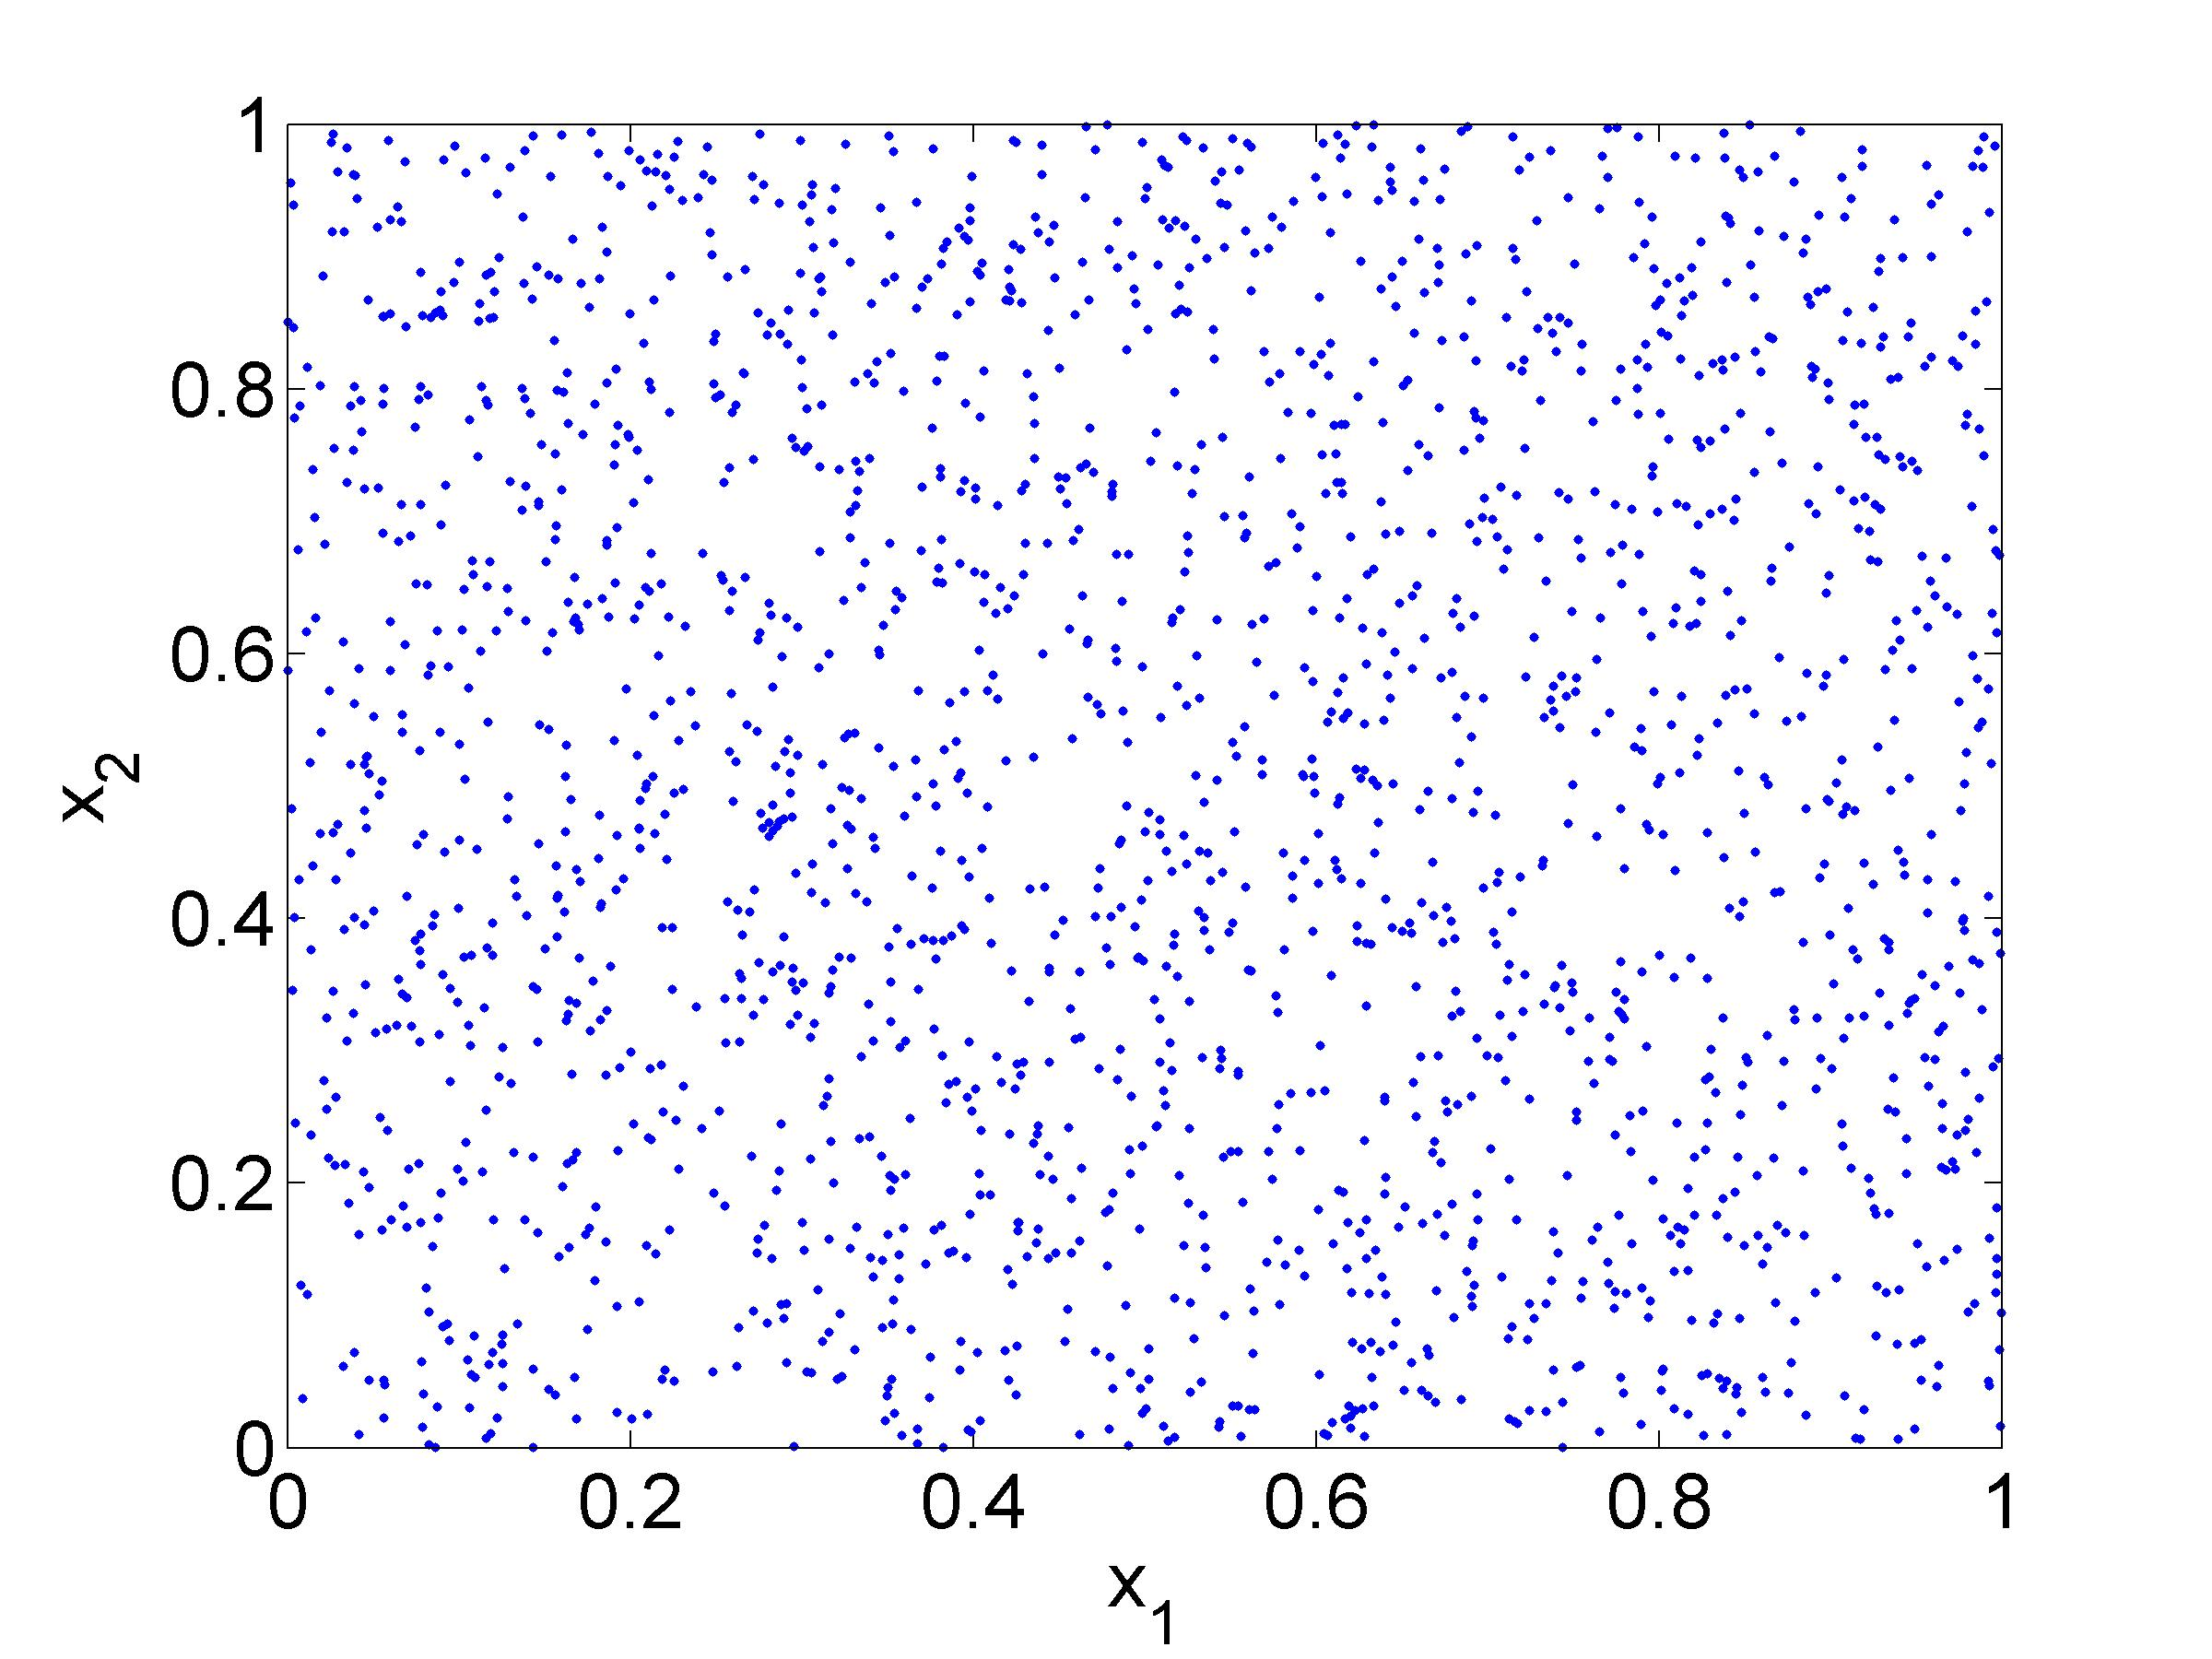
\includegraphics[width=0.5\textwidth]{xdata}
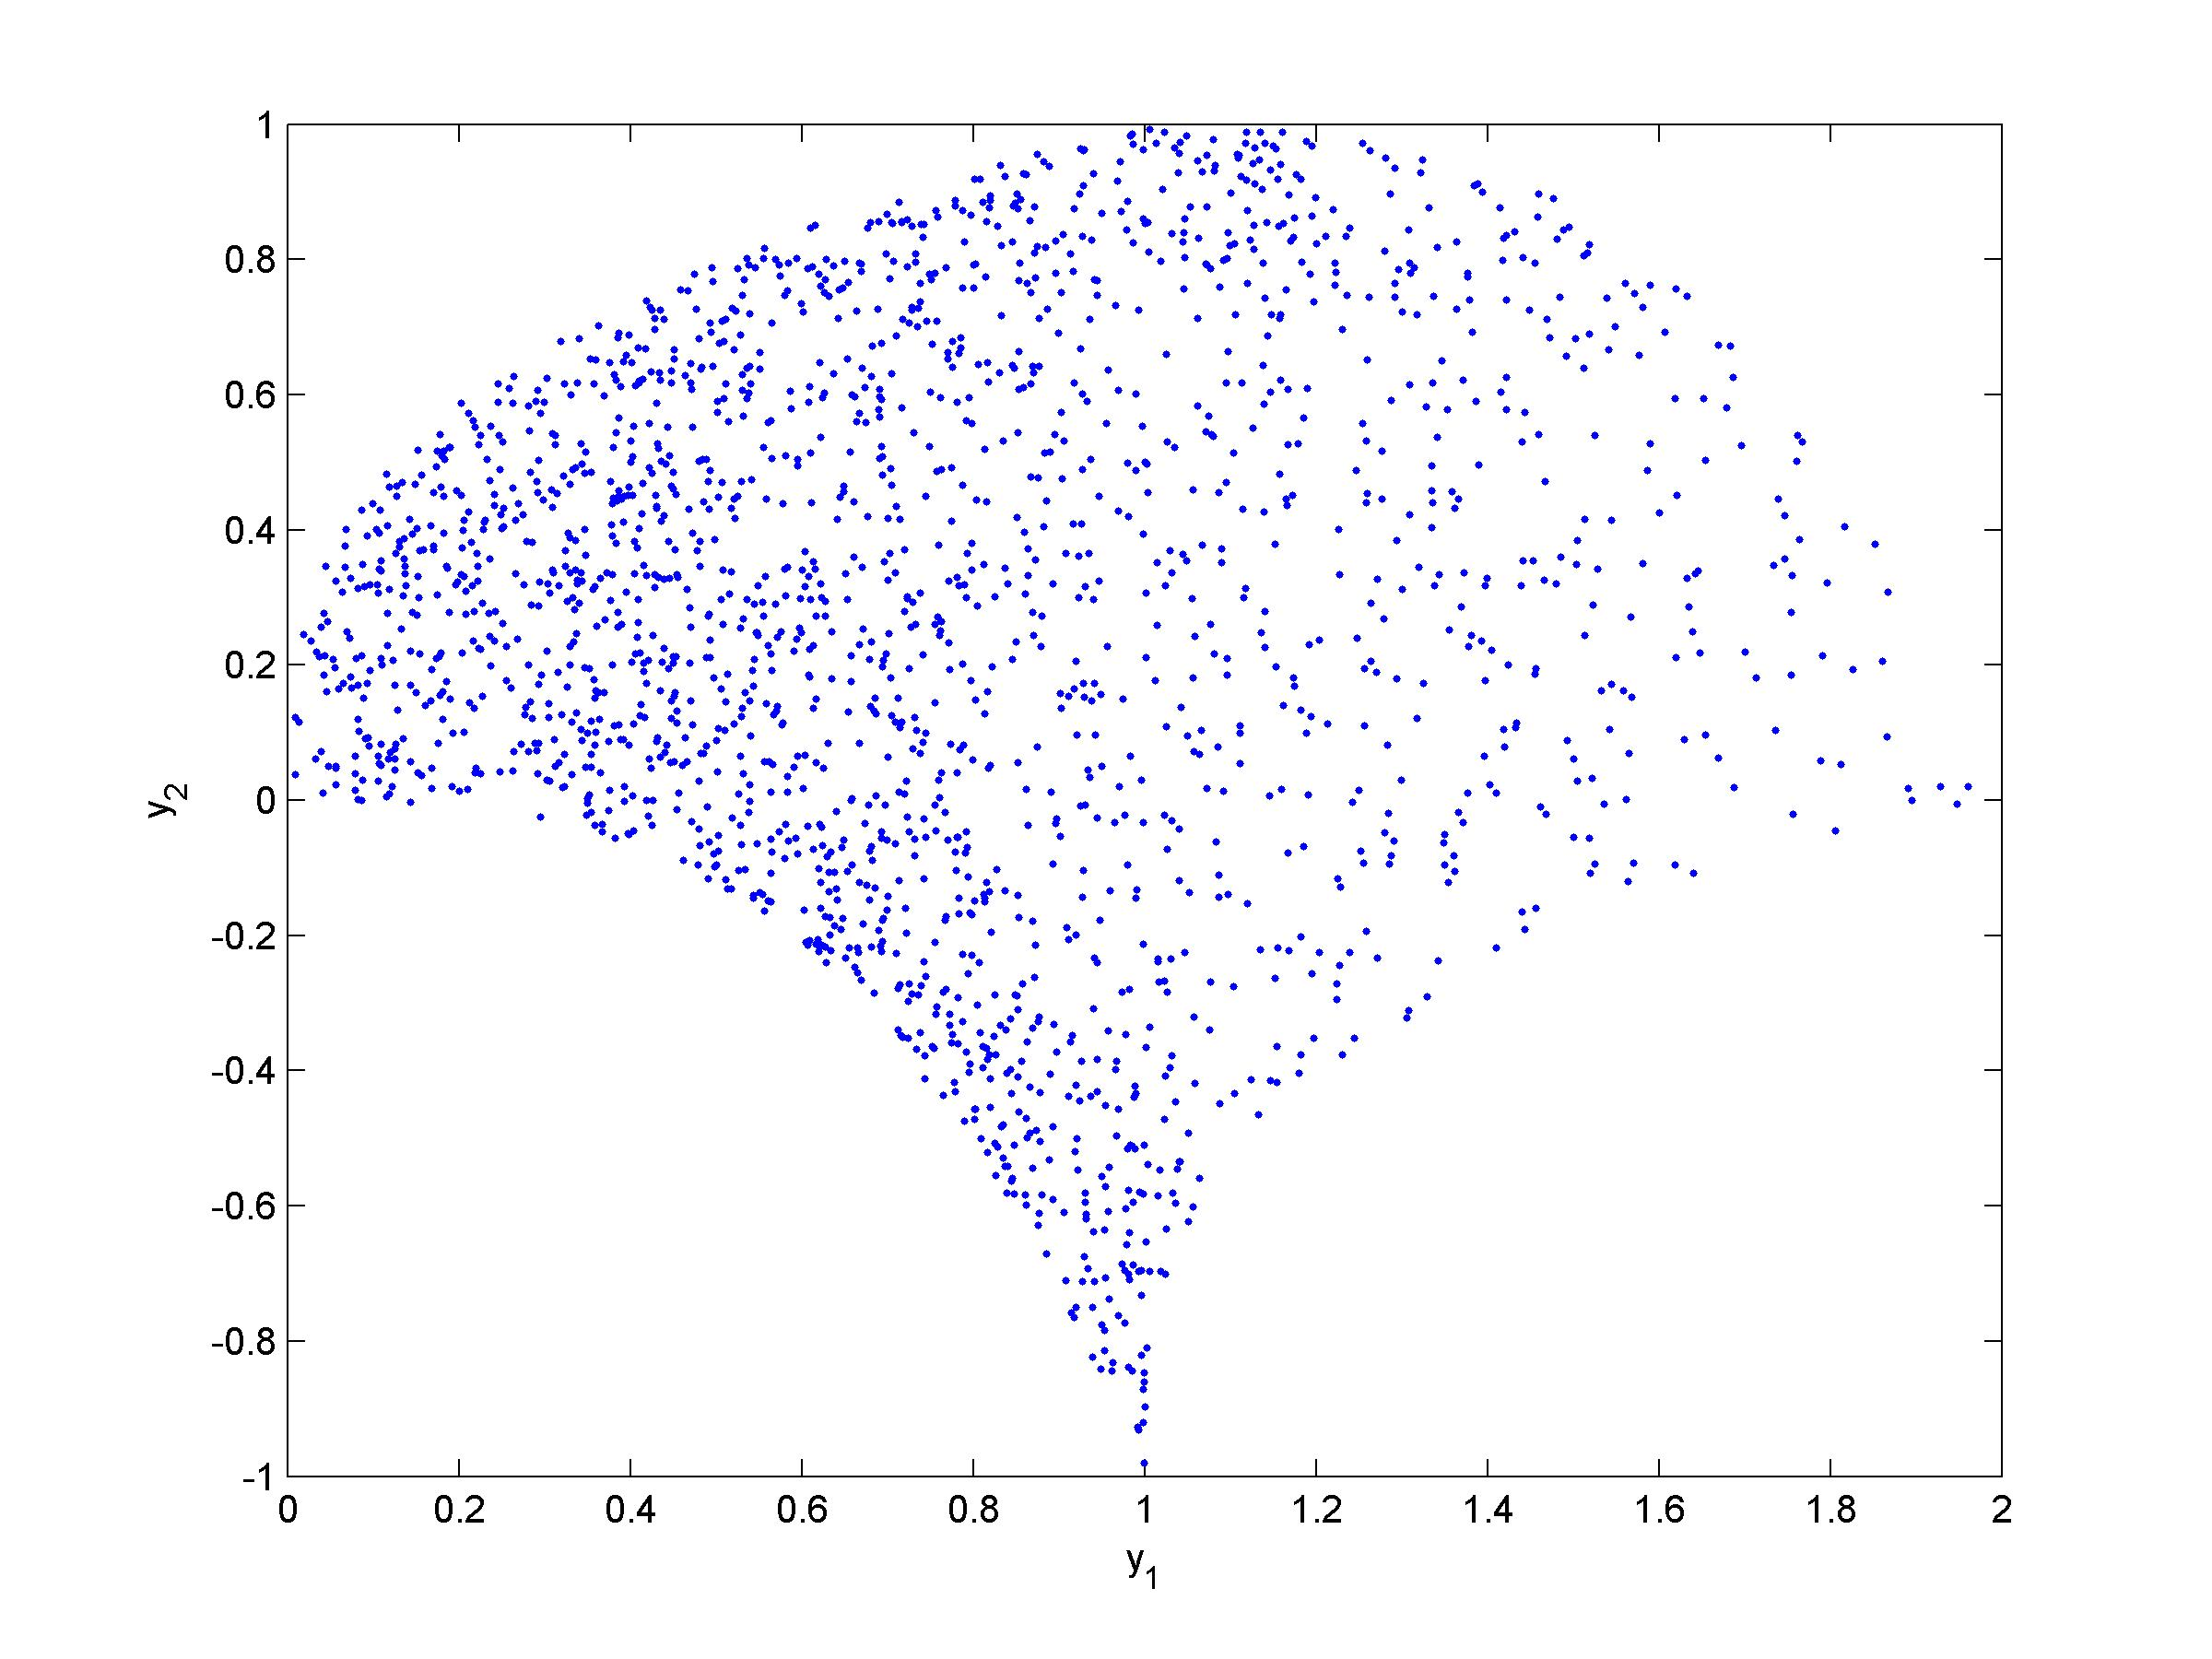
\includegraphics[width=0.5\textwidth]{ydata}
\caption{Left: data in ``true'' space. Right: data in ``ambient'' space.}
\label{fig:data}
\end{figure}

The results of doing DMAPS with the data $y_1, y_2$ are shown in in Figure \ref{fig:xdata_dmaps}.
%
Note that we do not recover the ``correct'' parameterization of the underlying variables $x_1, x_2$.

\begin{figure}[htb]
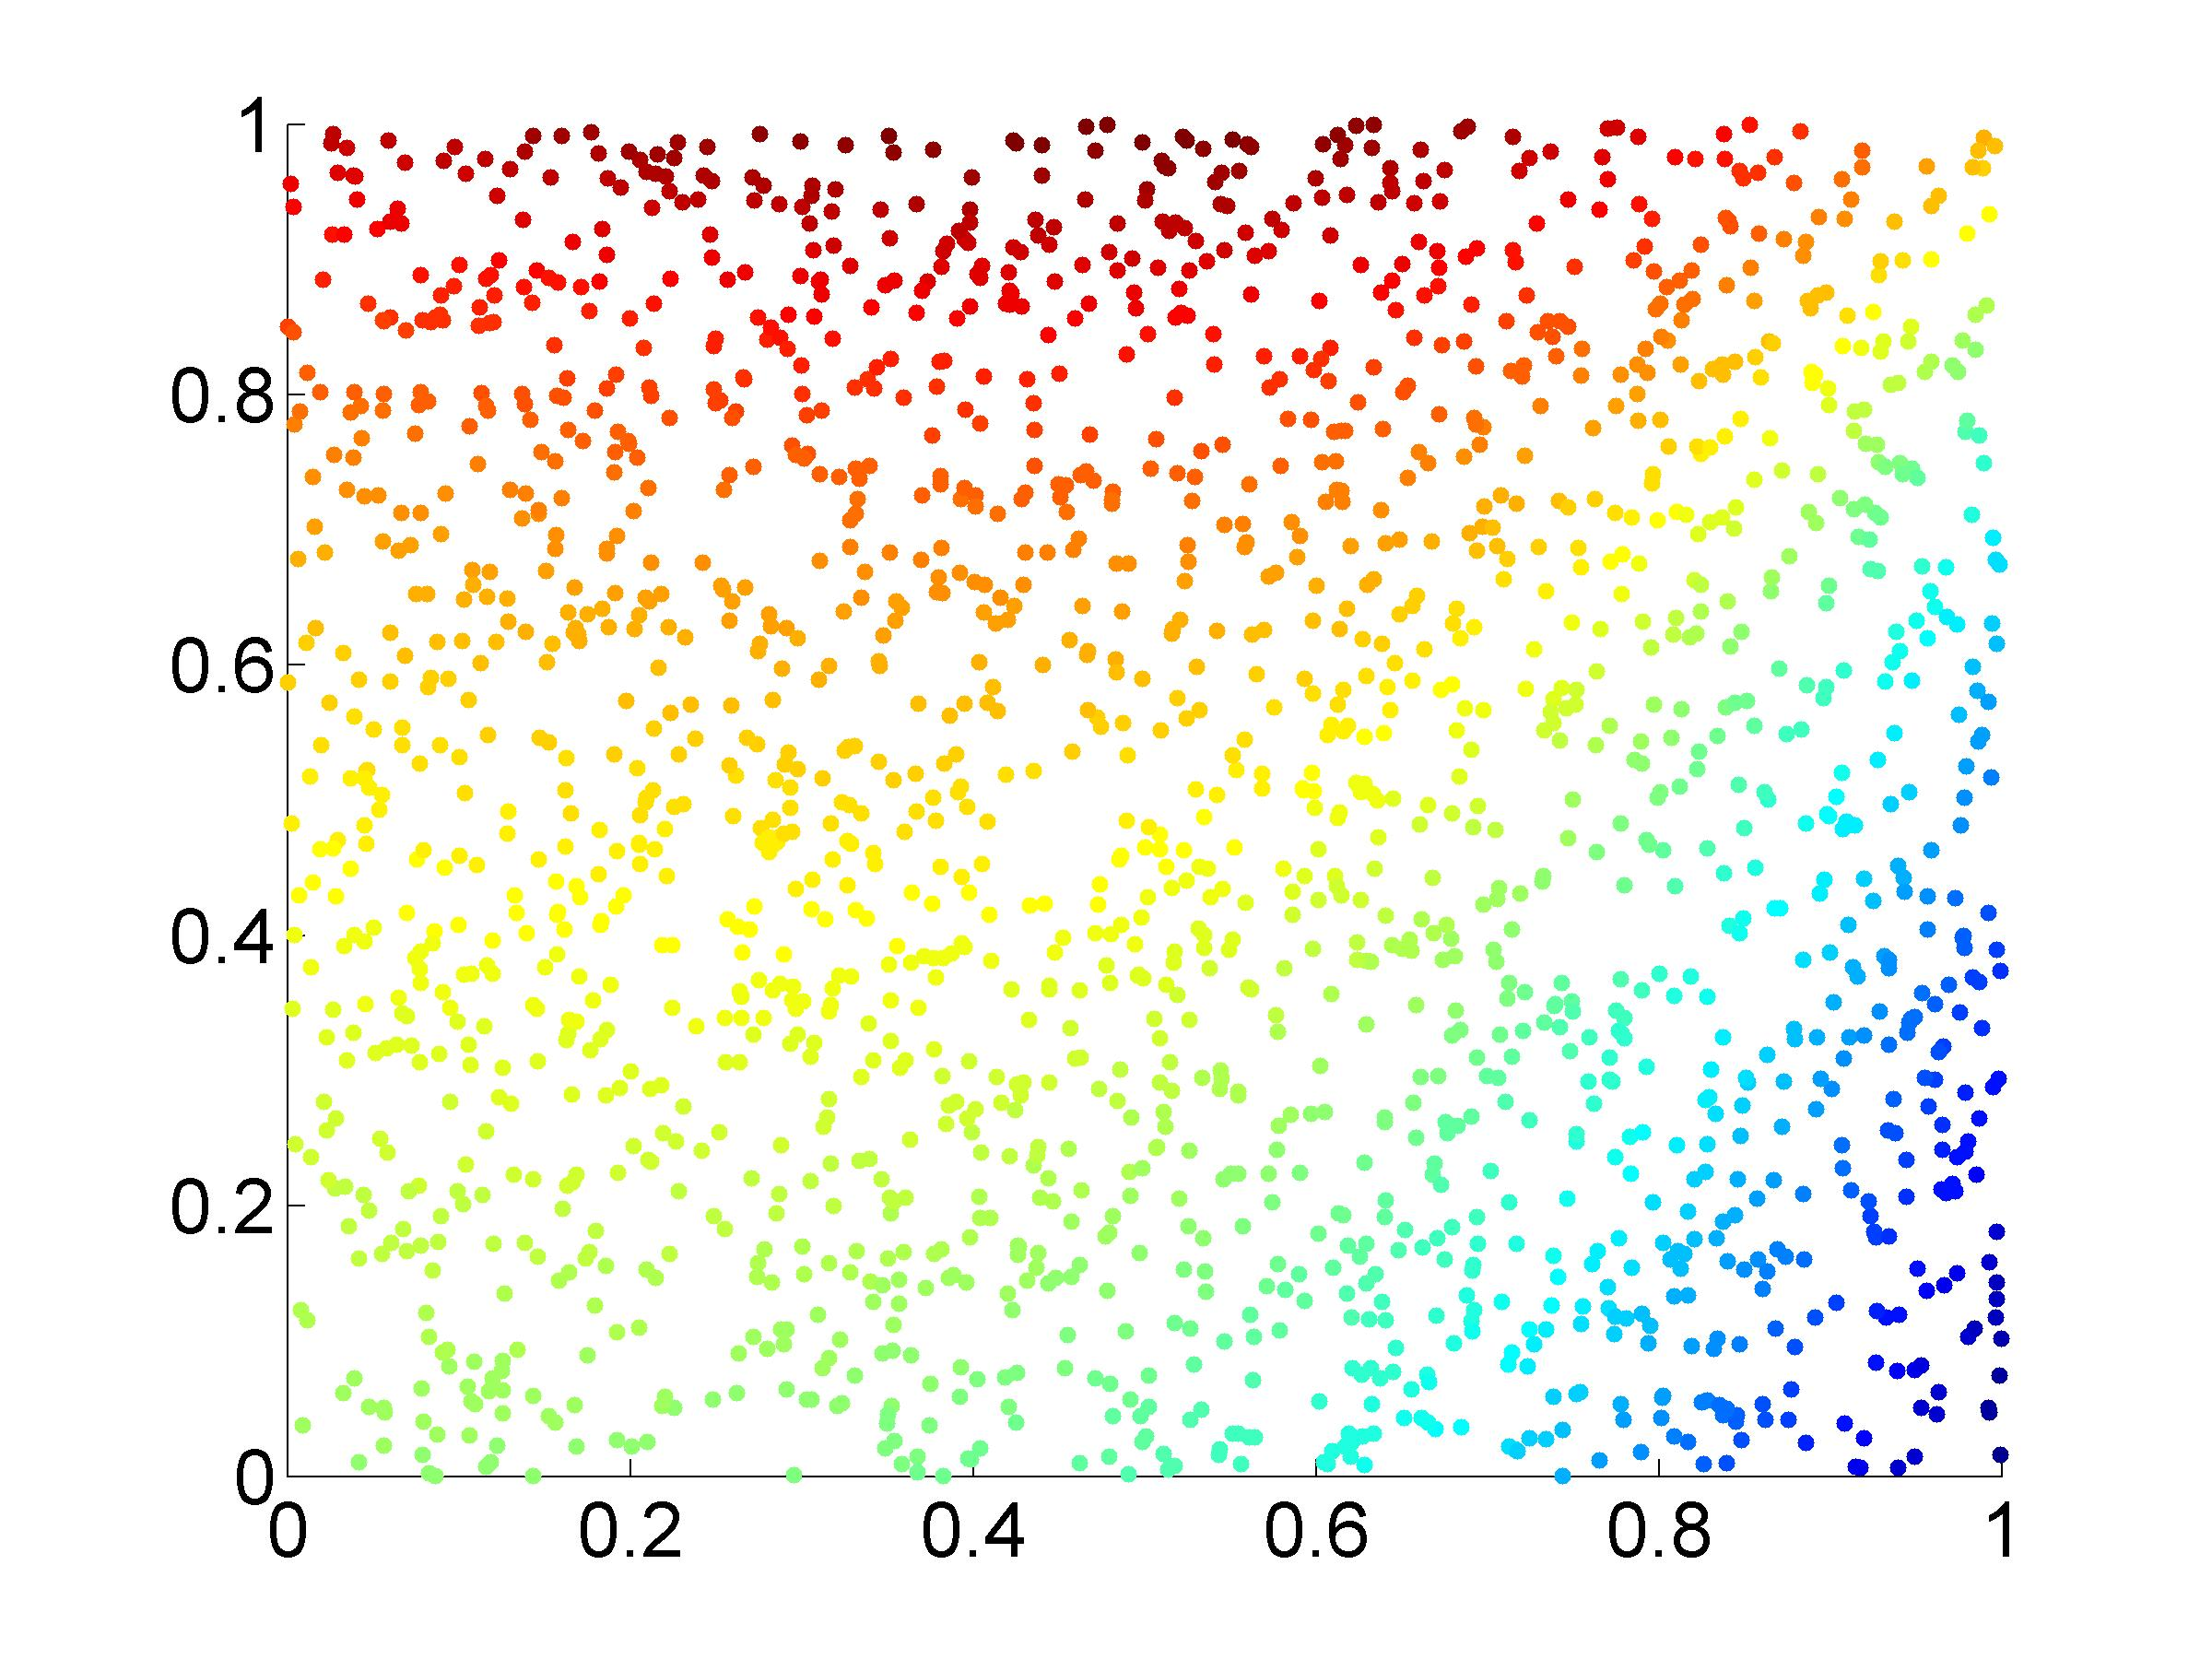
\includegraphics[width=0.5\textwidth]{xdata_colored_DMAPS1}
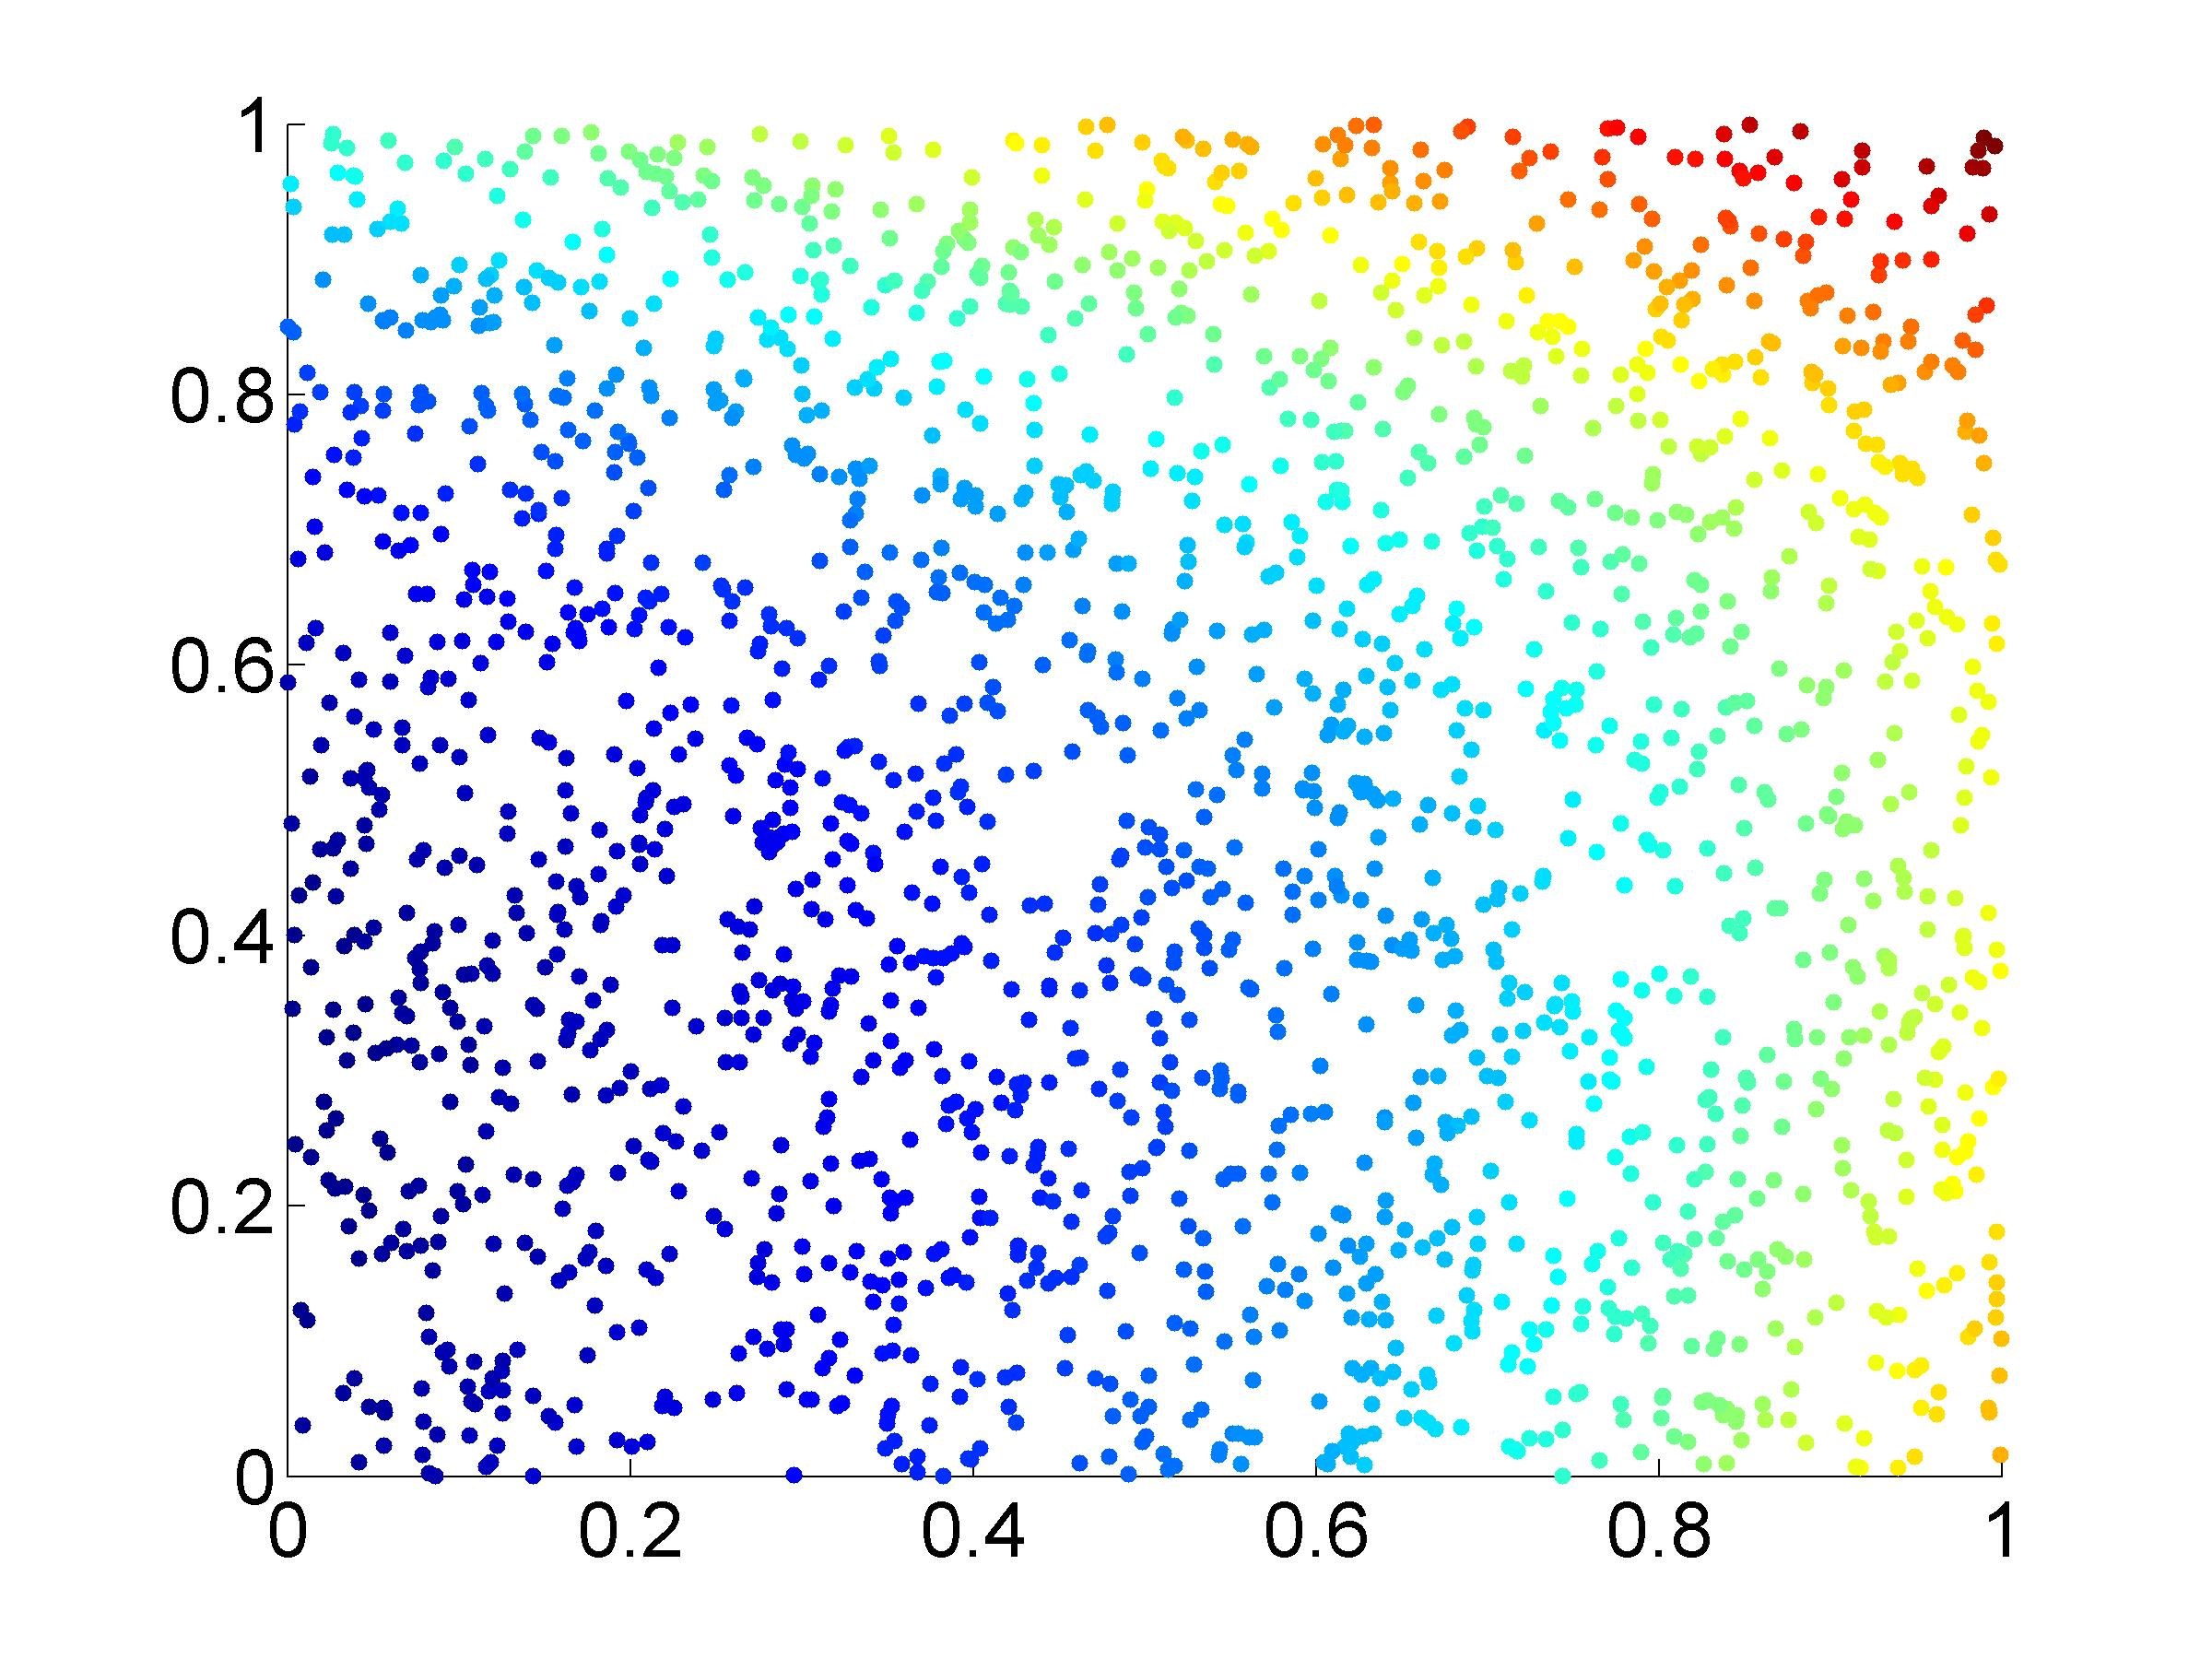
\includegraphics[width=0.5\textwidth]{xdata_colored_DMAPS2}
\caption{Data in ``true'' space ($x_1, x_2$), colored by the first (left) and second (right) nontrivial DMAPS component. The DMAPS embedding is computed from the data in the ``ambient'' space ($y_1, y_2$). Note that the parameterizationa we obtain are not the eigenfunctions that we expect for points sampled from the unit square.}
\label{fig:xdata_dmaps}
\end{figure}

If we do NIV with the data $y_1, y_2$, 
%taking our time windows so that the clouds around the points have standard deviation $1e-3$, 
we obtain the results in Figure \ref{fig:xdata_NIV}.
%
Note that we now recover the ``correct'' variables.

\begin{figure}[htb]
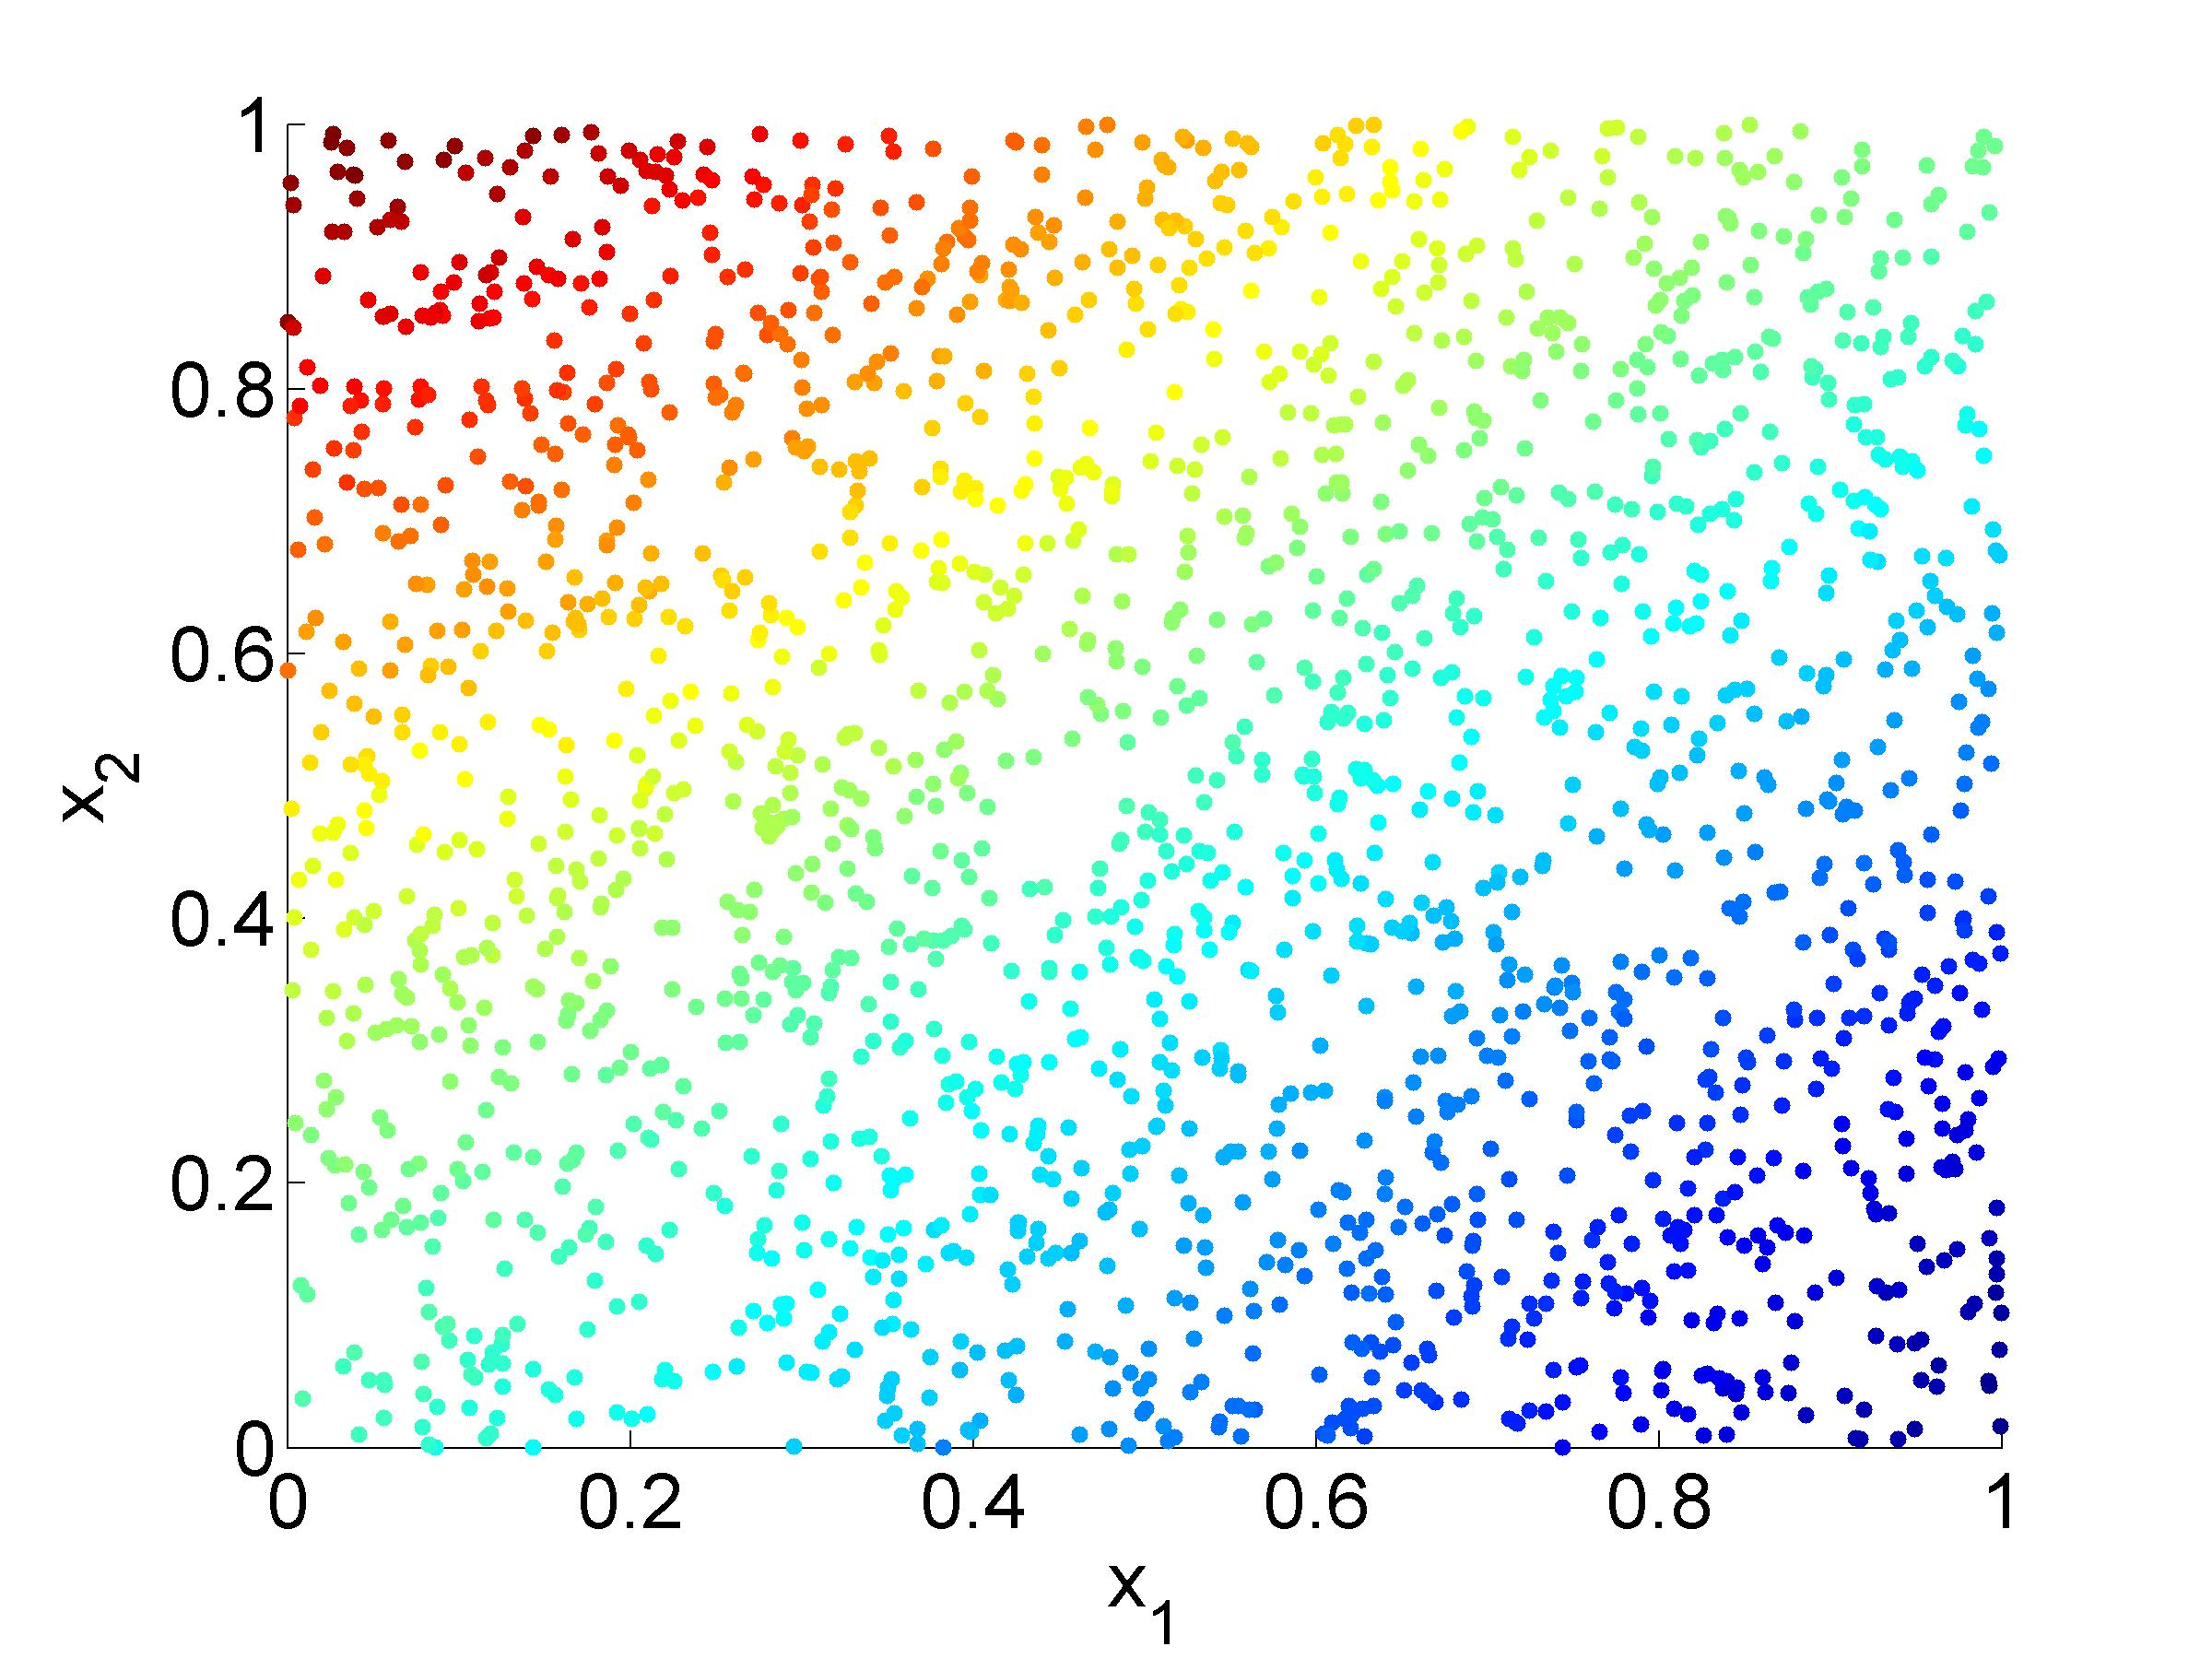
\includegraphics[width=0.5\textwidth]{xdata_colored_NIV1}
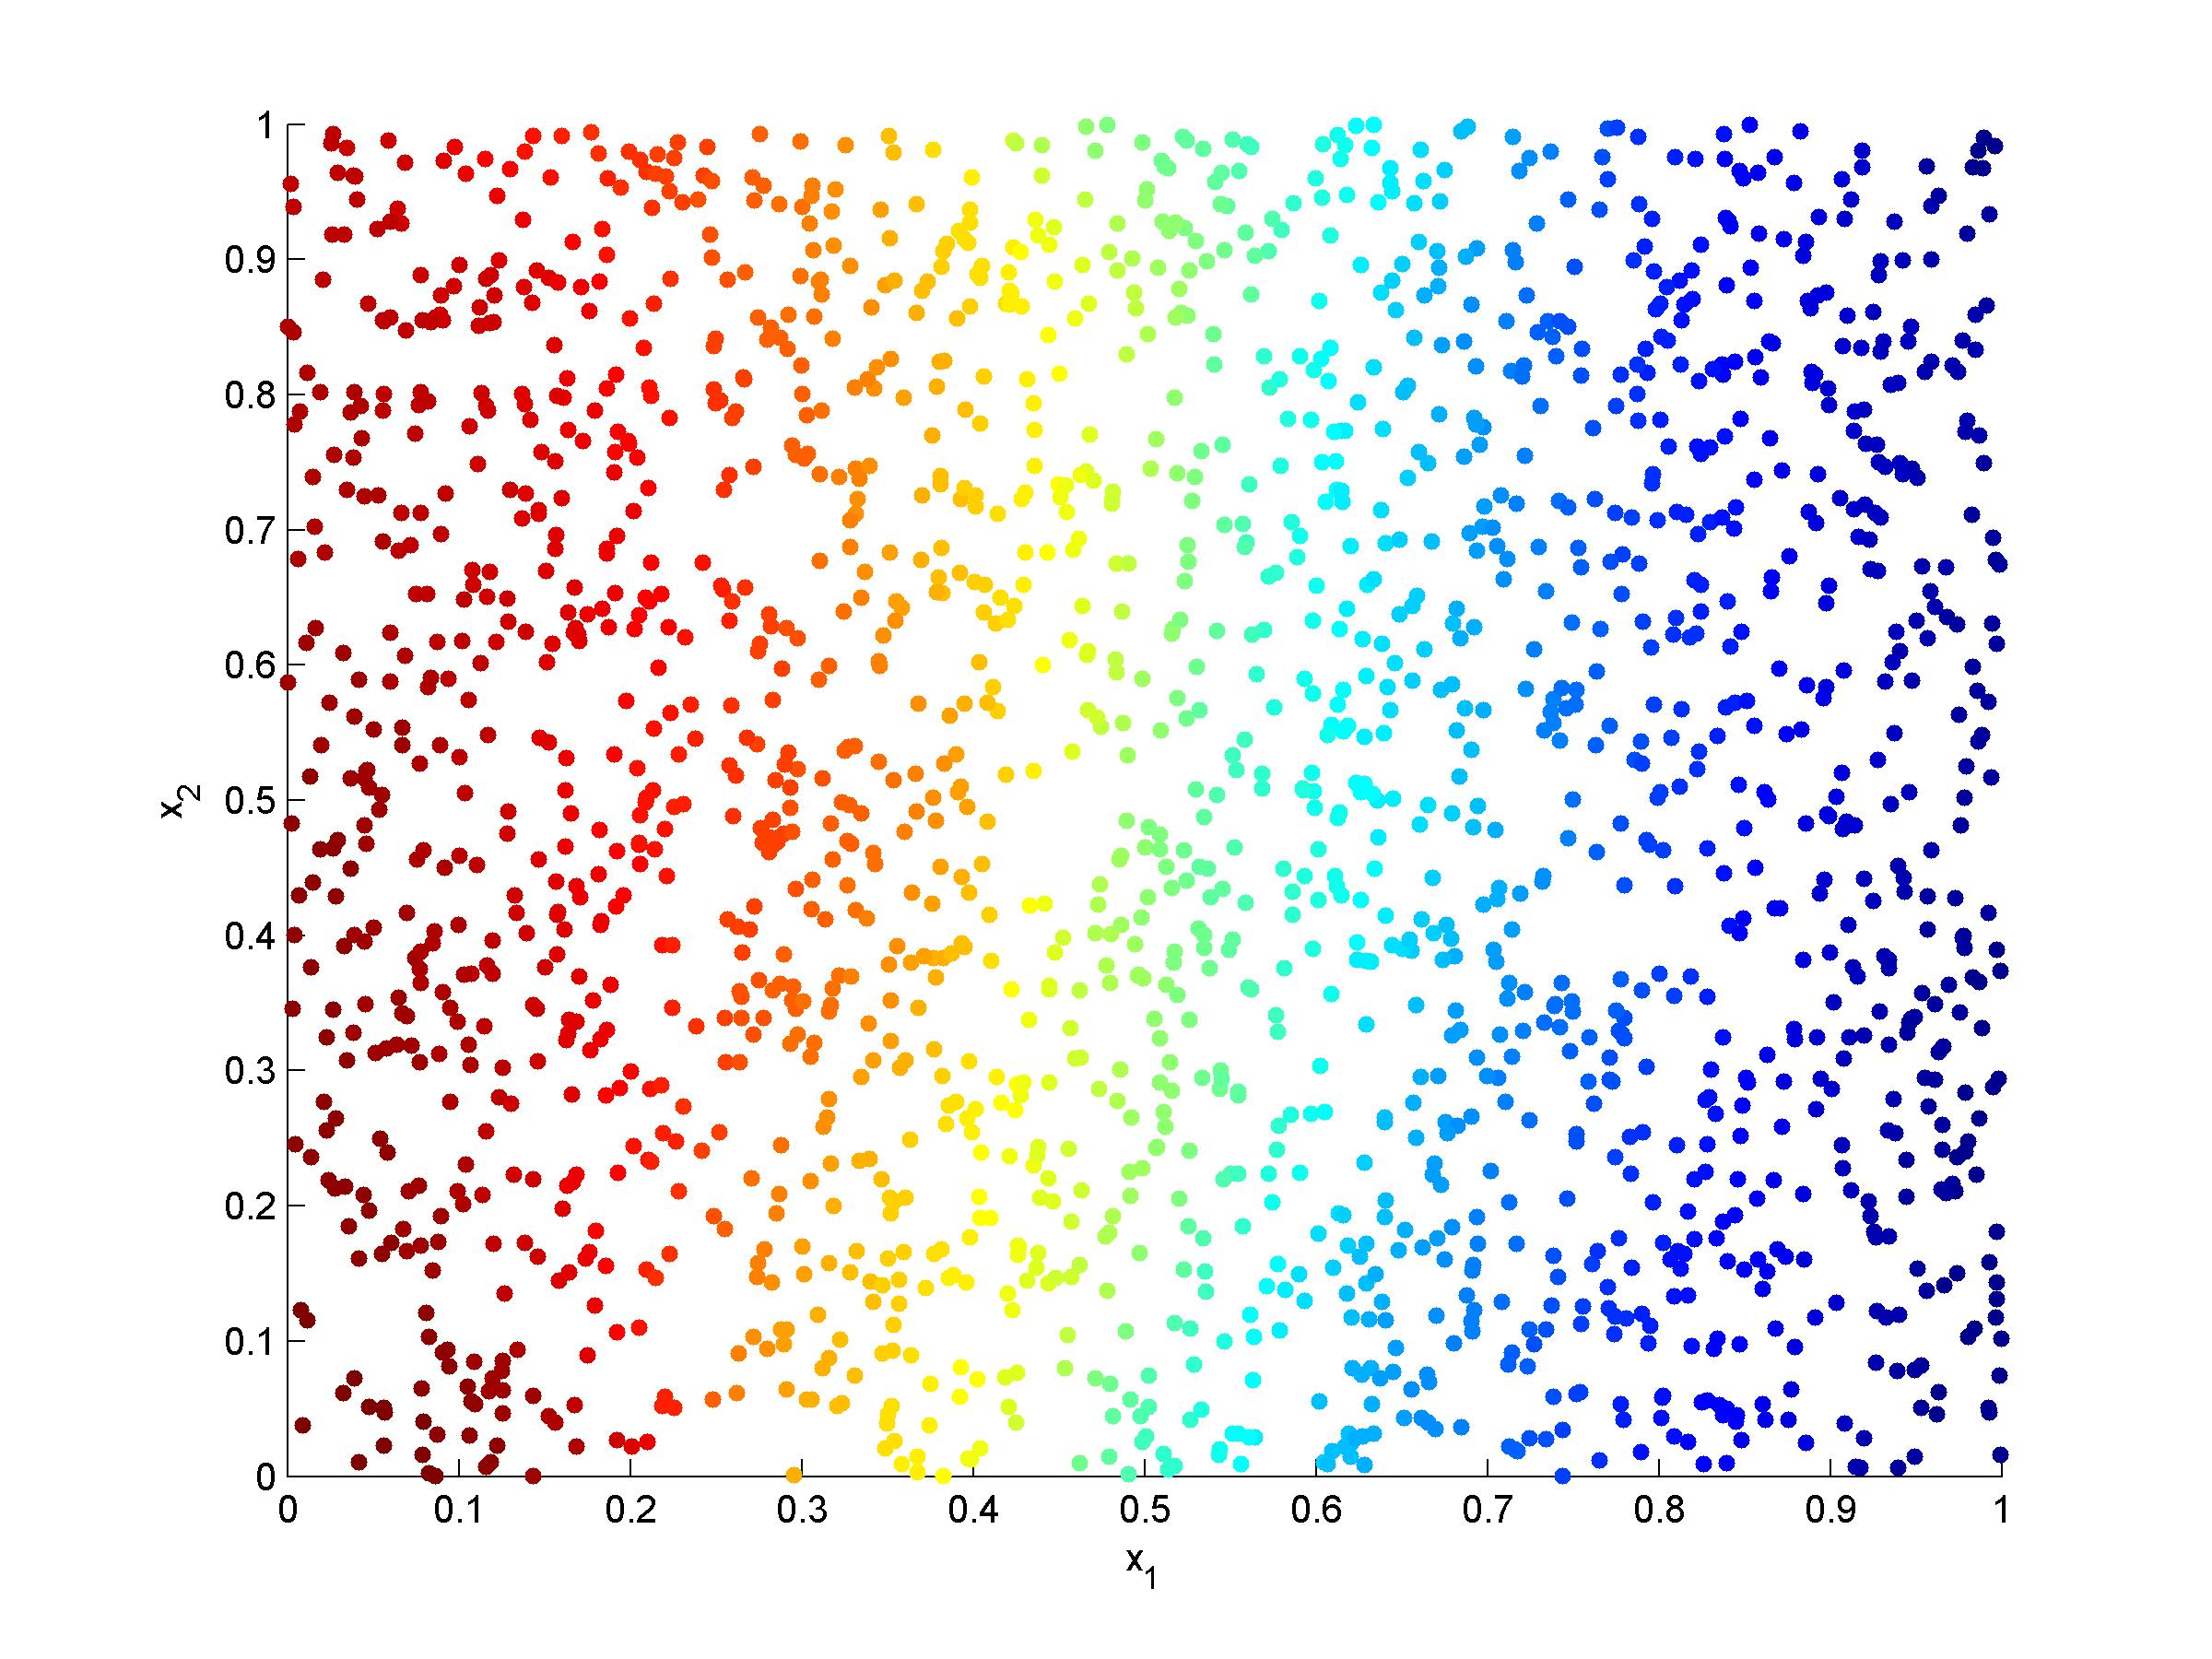
\includegraphics[width=0.5\textwidth]{xdata_colored_NIV2}
\caption{Data in ``true'' space ($x_1, x_2$), colored by the first (left) and second (right) nontrivial NIV. The NIV embedding is computed from the data in the ambient space ($y_1, y_2$), with clouds around the points have standard deviation $1e-3$. Note that the parameterizations we obtain are the eigenfunctions that we expect for points sampled from the unit square.}
\label{fig:xdata_NIV}
\end{figure}

We now look at the effect of adding additional noise to our system.
%
Consider adding white Gaussian noise to the $y_1, y_2$ data
\begin{eqnarray}
z_1 & = & x_1 + x_2^3 + \xi_1 \\
z_2 & = & x_2 - x_1^3 + \xi_2 \\
z_3 & = & \xi_3
\end{eqnarray}
where $\xi_1, \xi_2, \xi_3 \sim \mathcal{N}(0, \sigma^2)$

If $\sigma = 0.01$ (so the added noise is much smaller than the noise in the original clouds), we obtain a parameterization shown in Figure \ref{fig:xdata_NIV_noise1} using NIV.

\begin{figure}[htb]
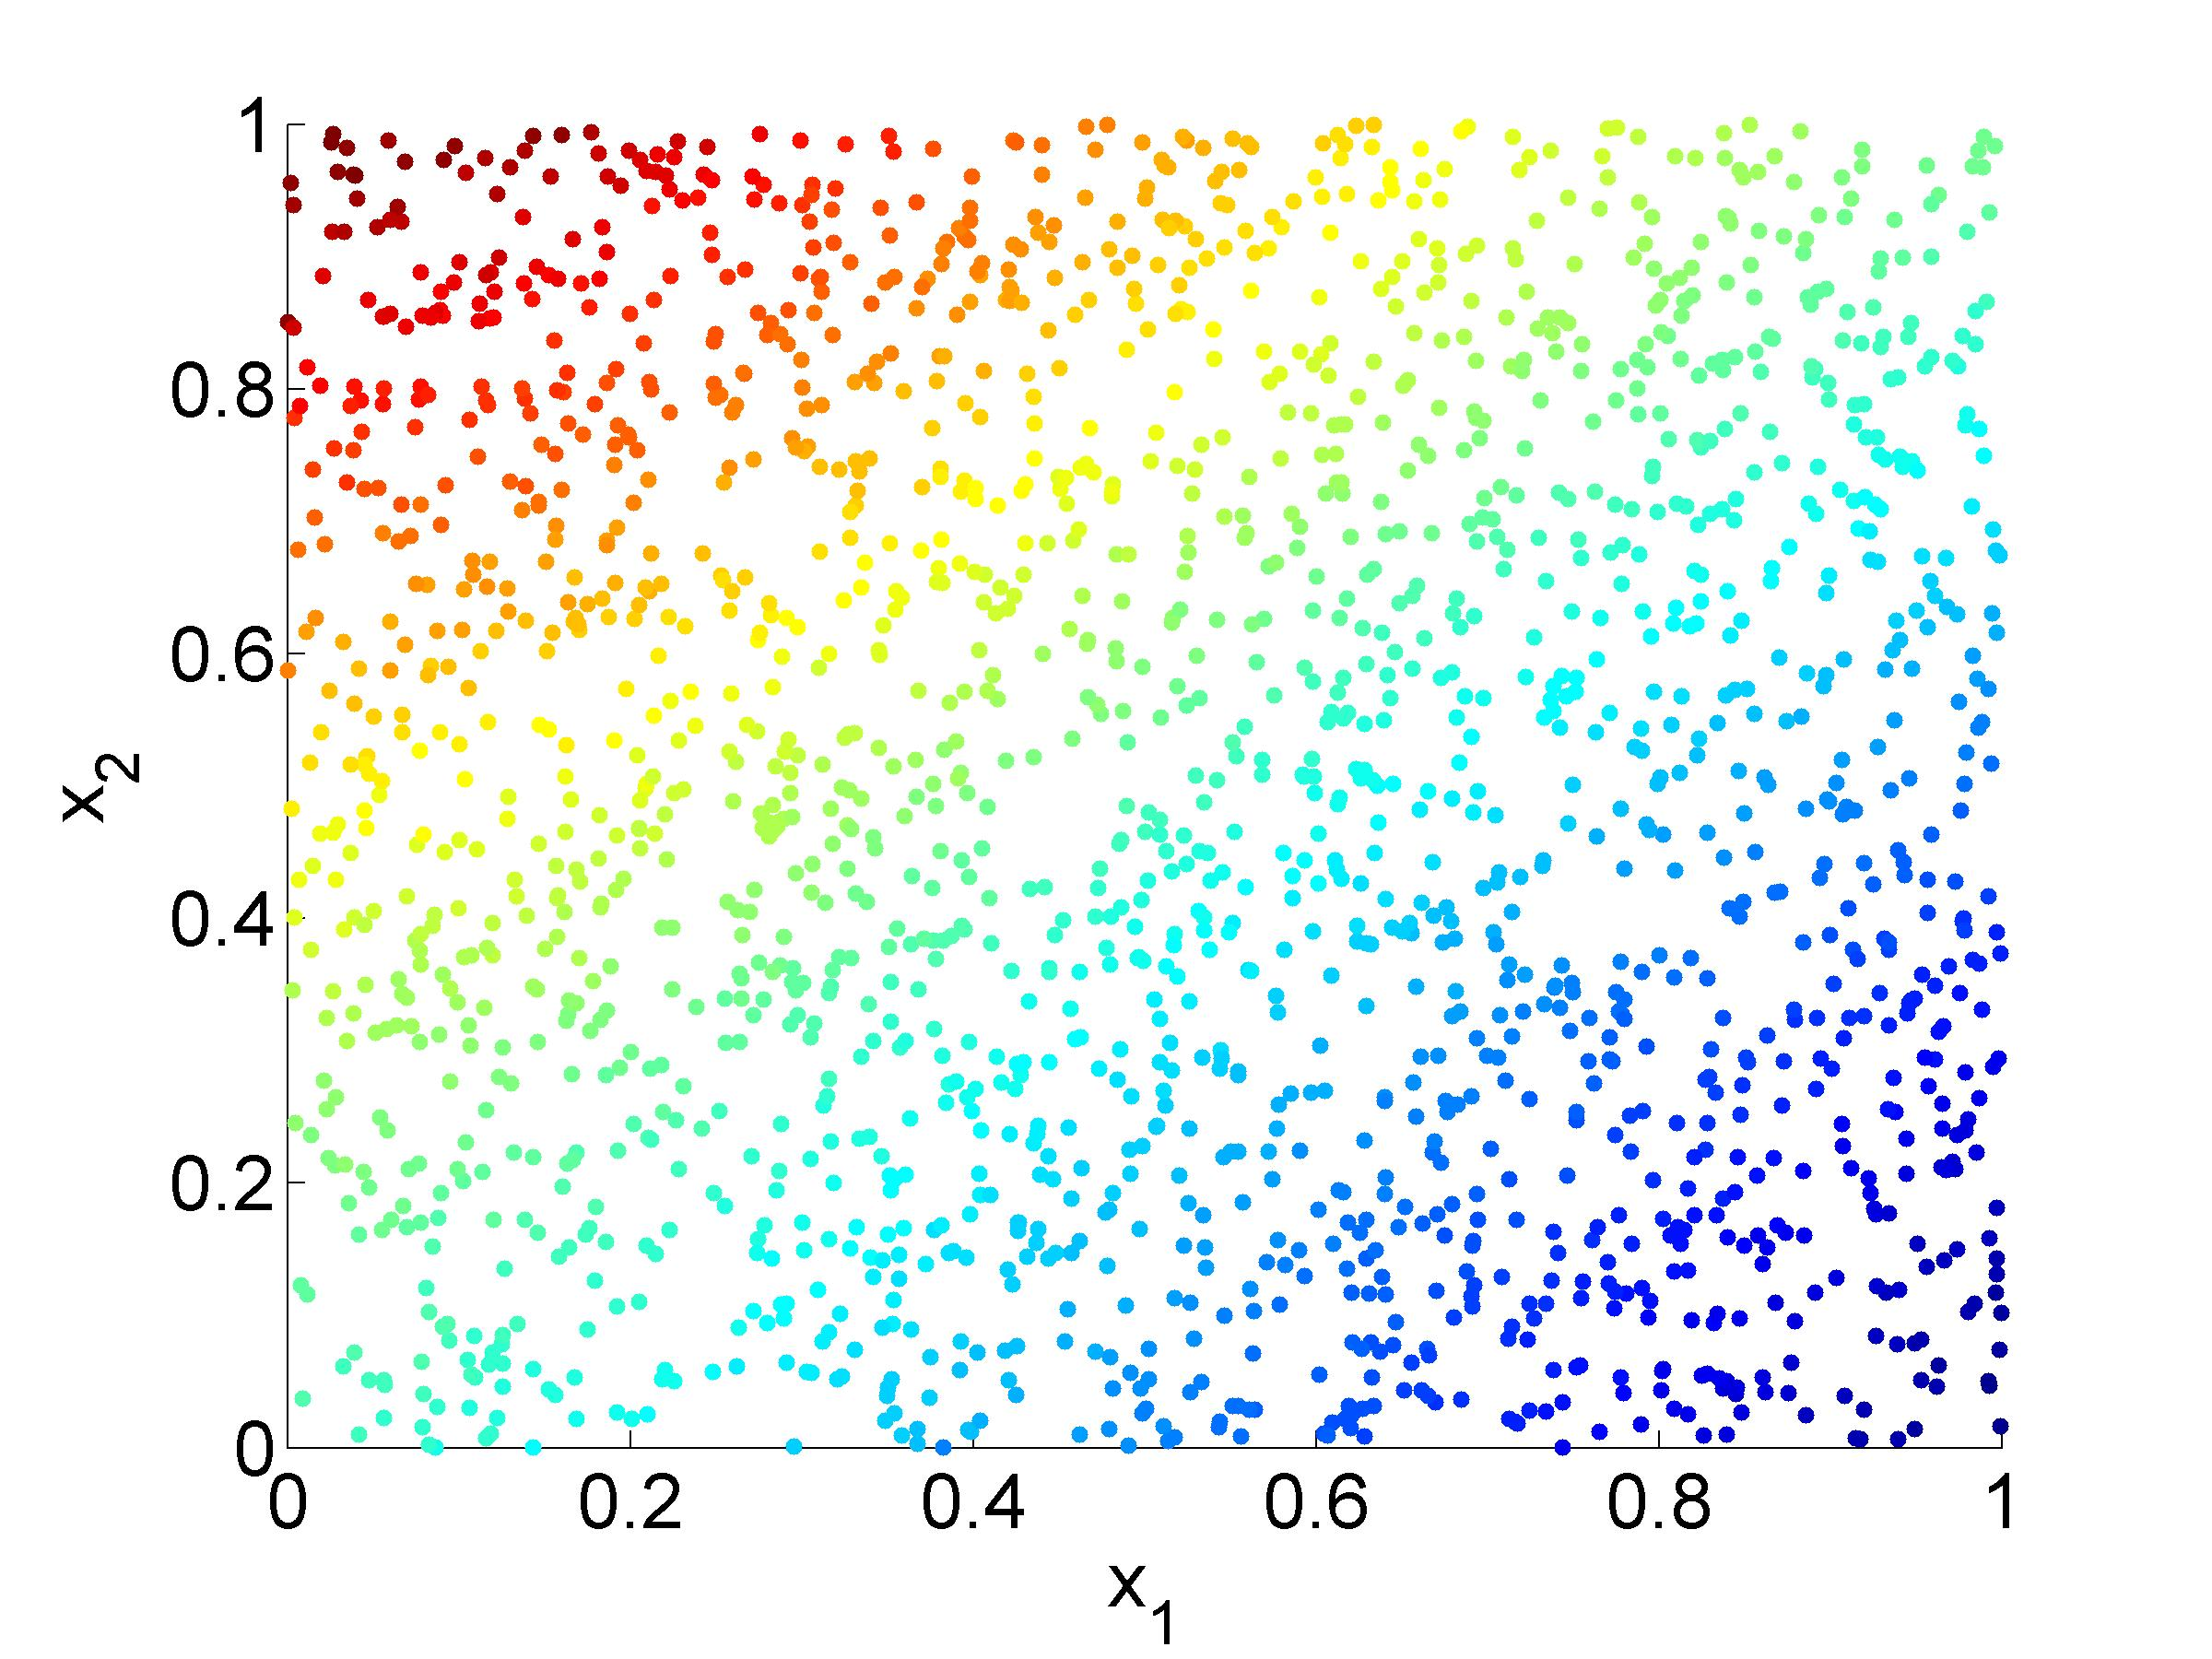
\includegraphics[width=0.5\textwidth]{xdata_noise1_colored_NIV1}
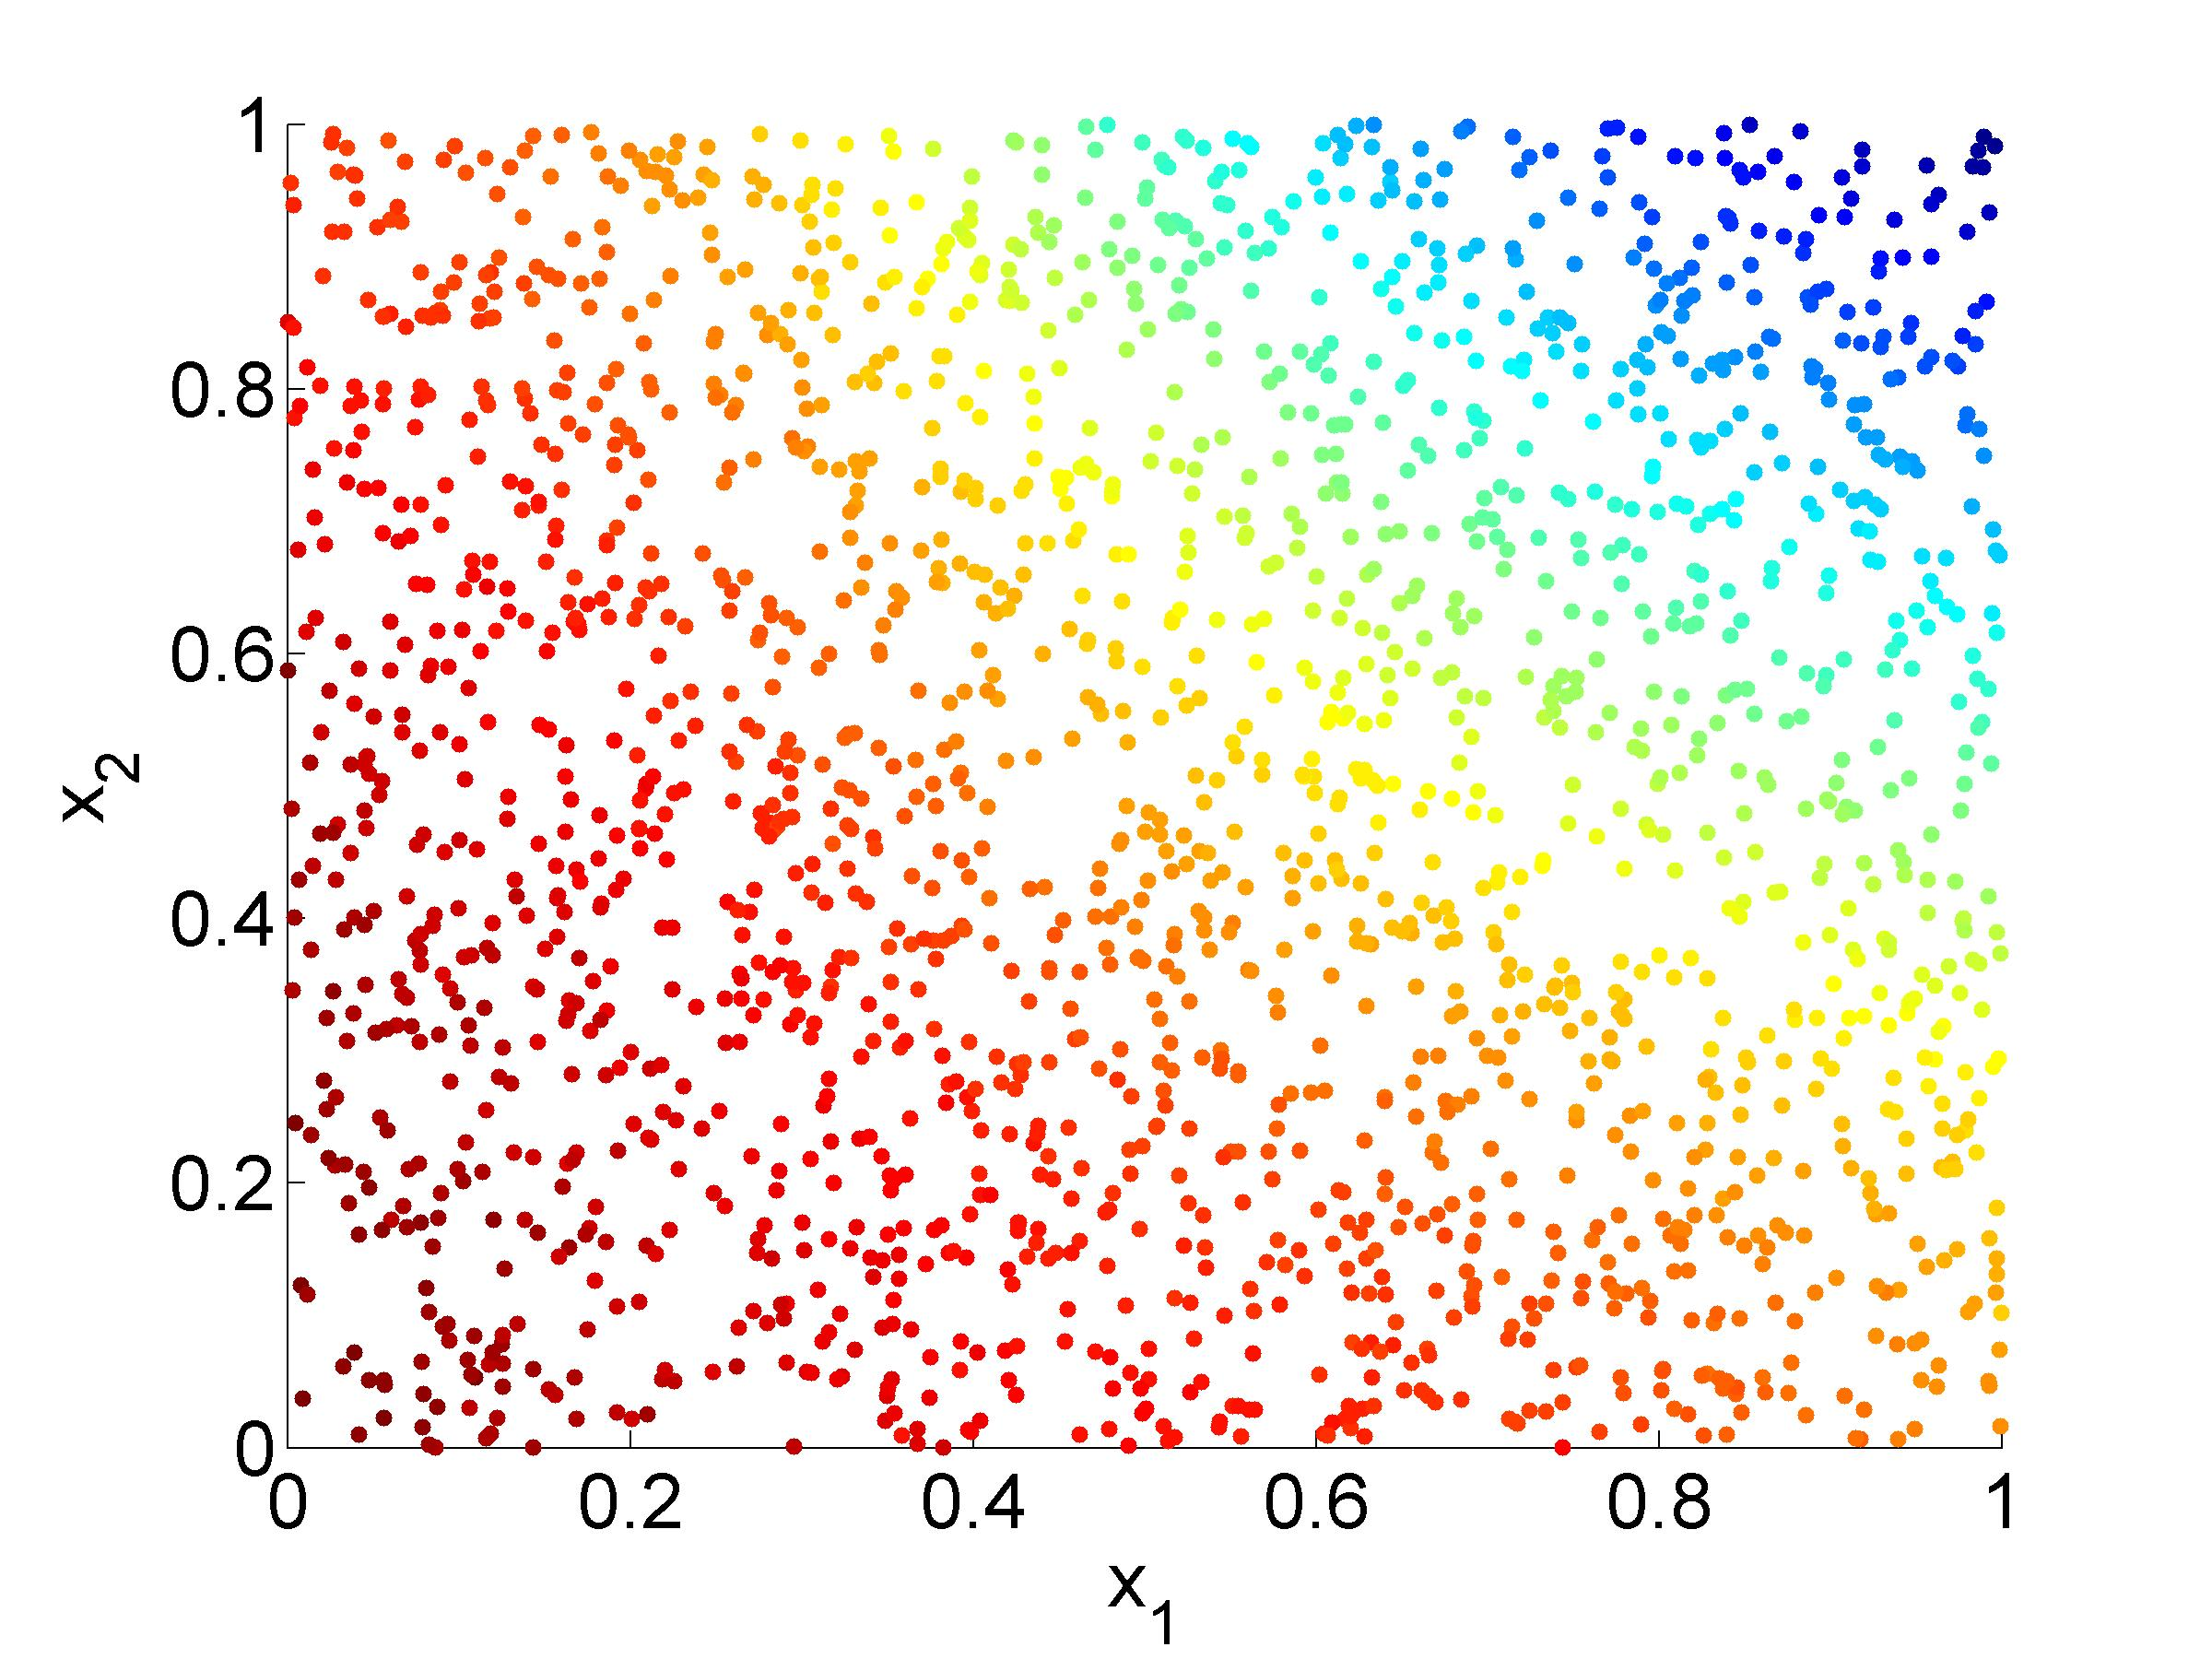
\includegraphics[width=0.5\textwidth]{xdata_noise1_colored_NIV2}
\caption{Data in ``true'' space ($x_1, x_2$), colored by the first (left) and second (right) nontrivial NIV. The NIV embedding is computed from the data in the ambient space with added noise ($z_1, z_2$, with $\sigma = 0.01$). Note that the parameterizations we obtain are the eigenfunctions that we expect for points sampled from the unit square.}
\label{fig:xdata_NIV_noise1}
\end{figure}

If $\sigma = 100$ (so the added noise is much larger than the noise in the original clouds), we obtain a parameterization shown in Figure \ref{fig:xdata_NIV_noise2} using NIV.

\begin{figure}[htb]
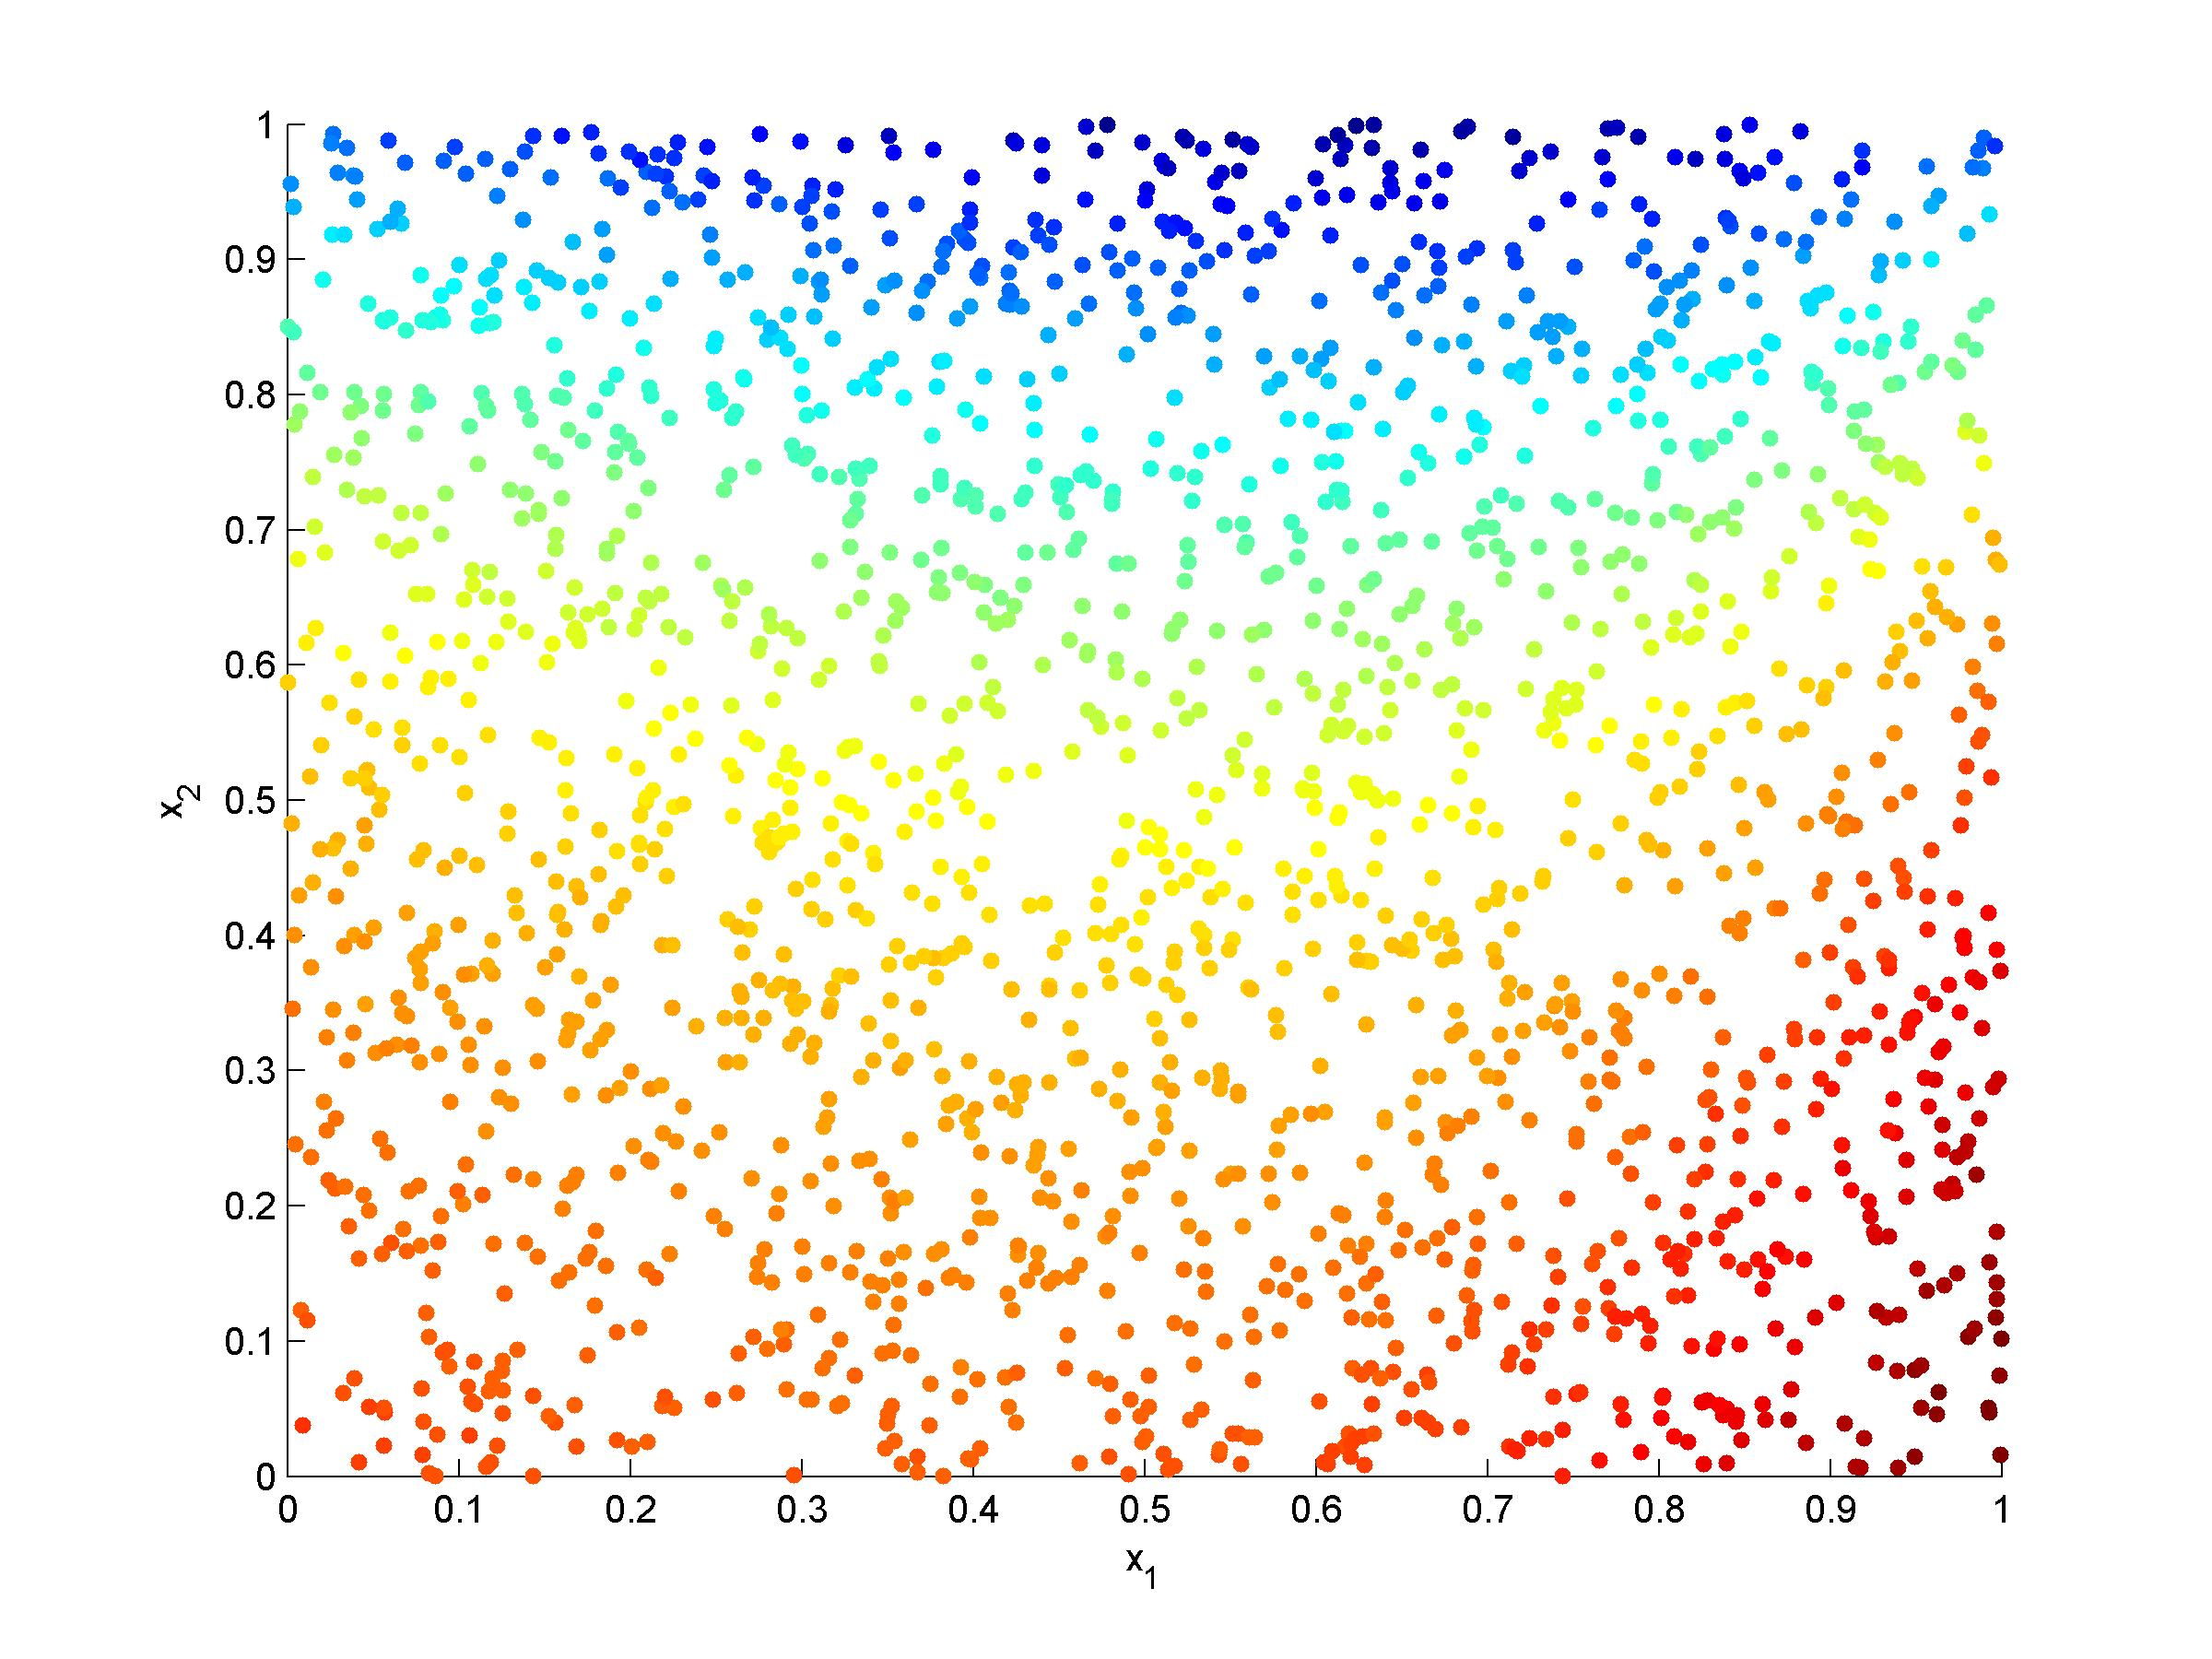
\includegraphics[width=0.5\textwidth]{xdata_noise2_colored_NIV1}
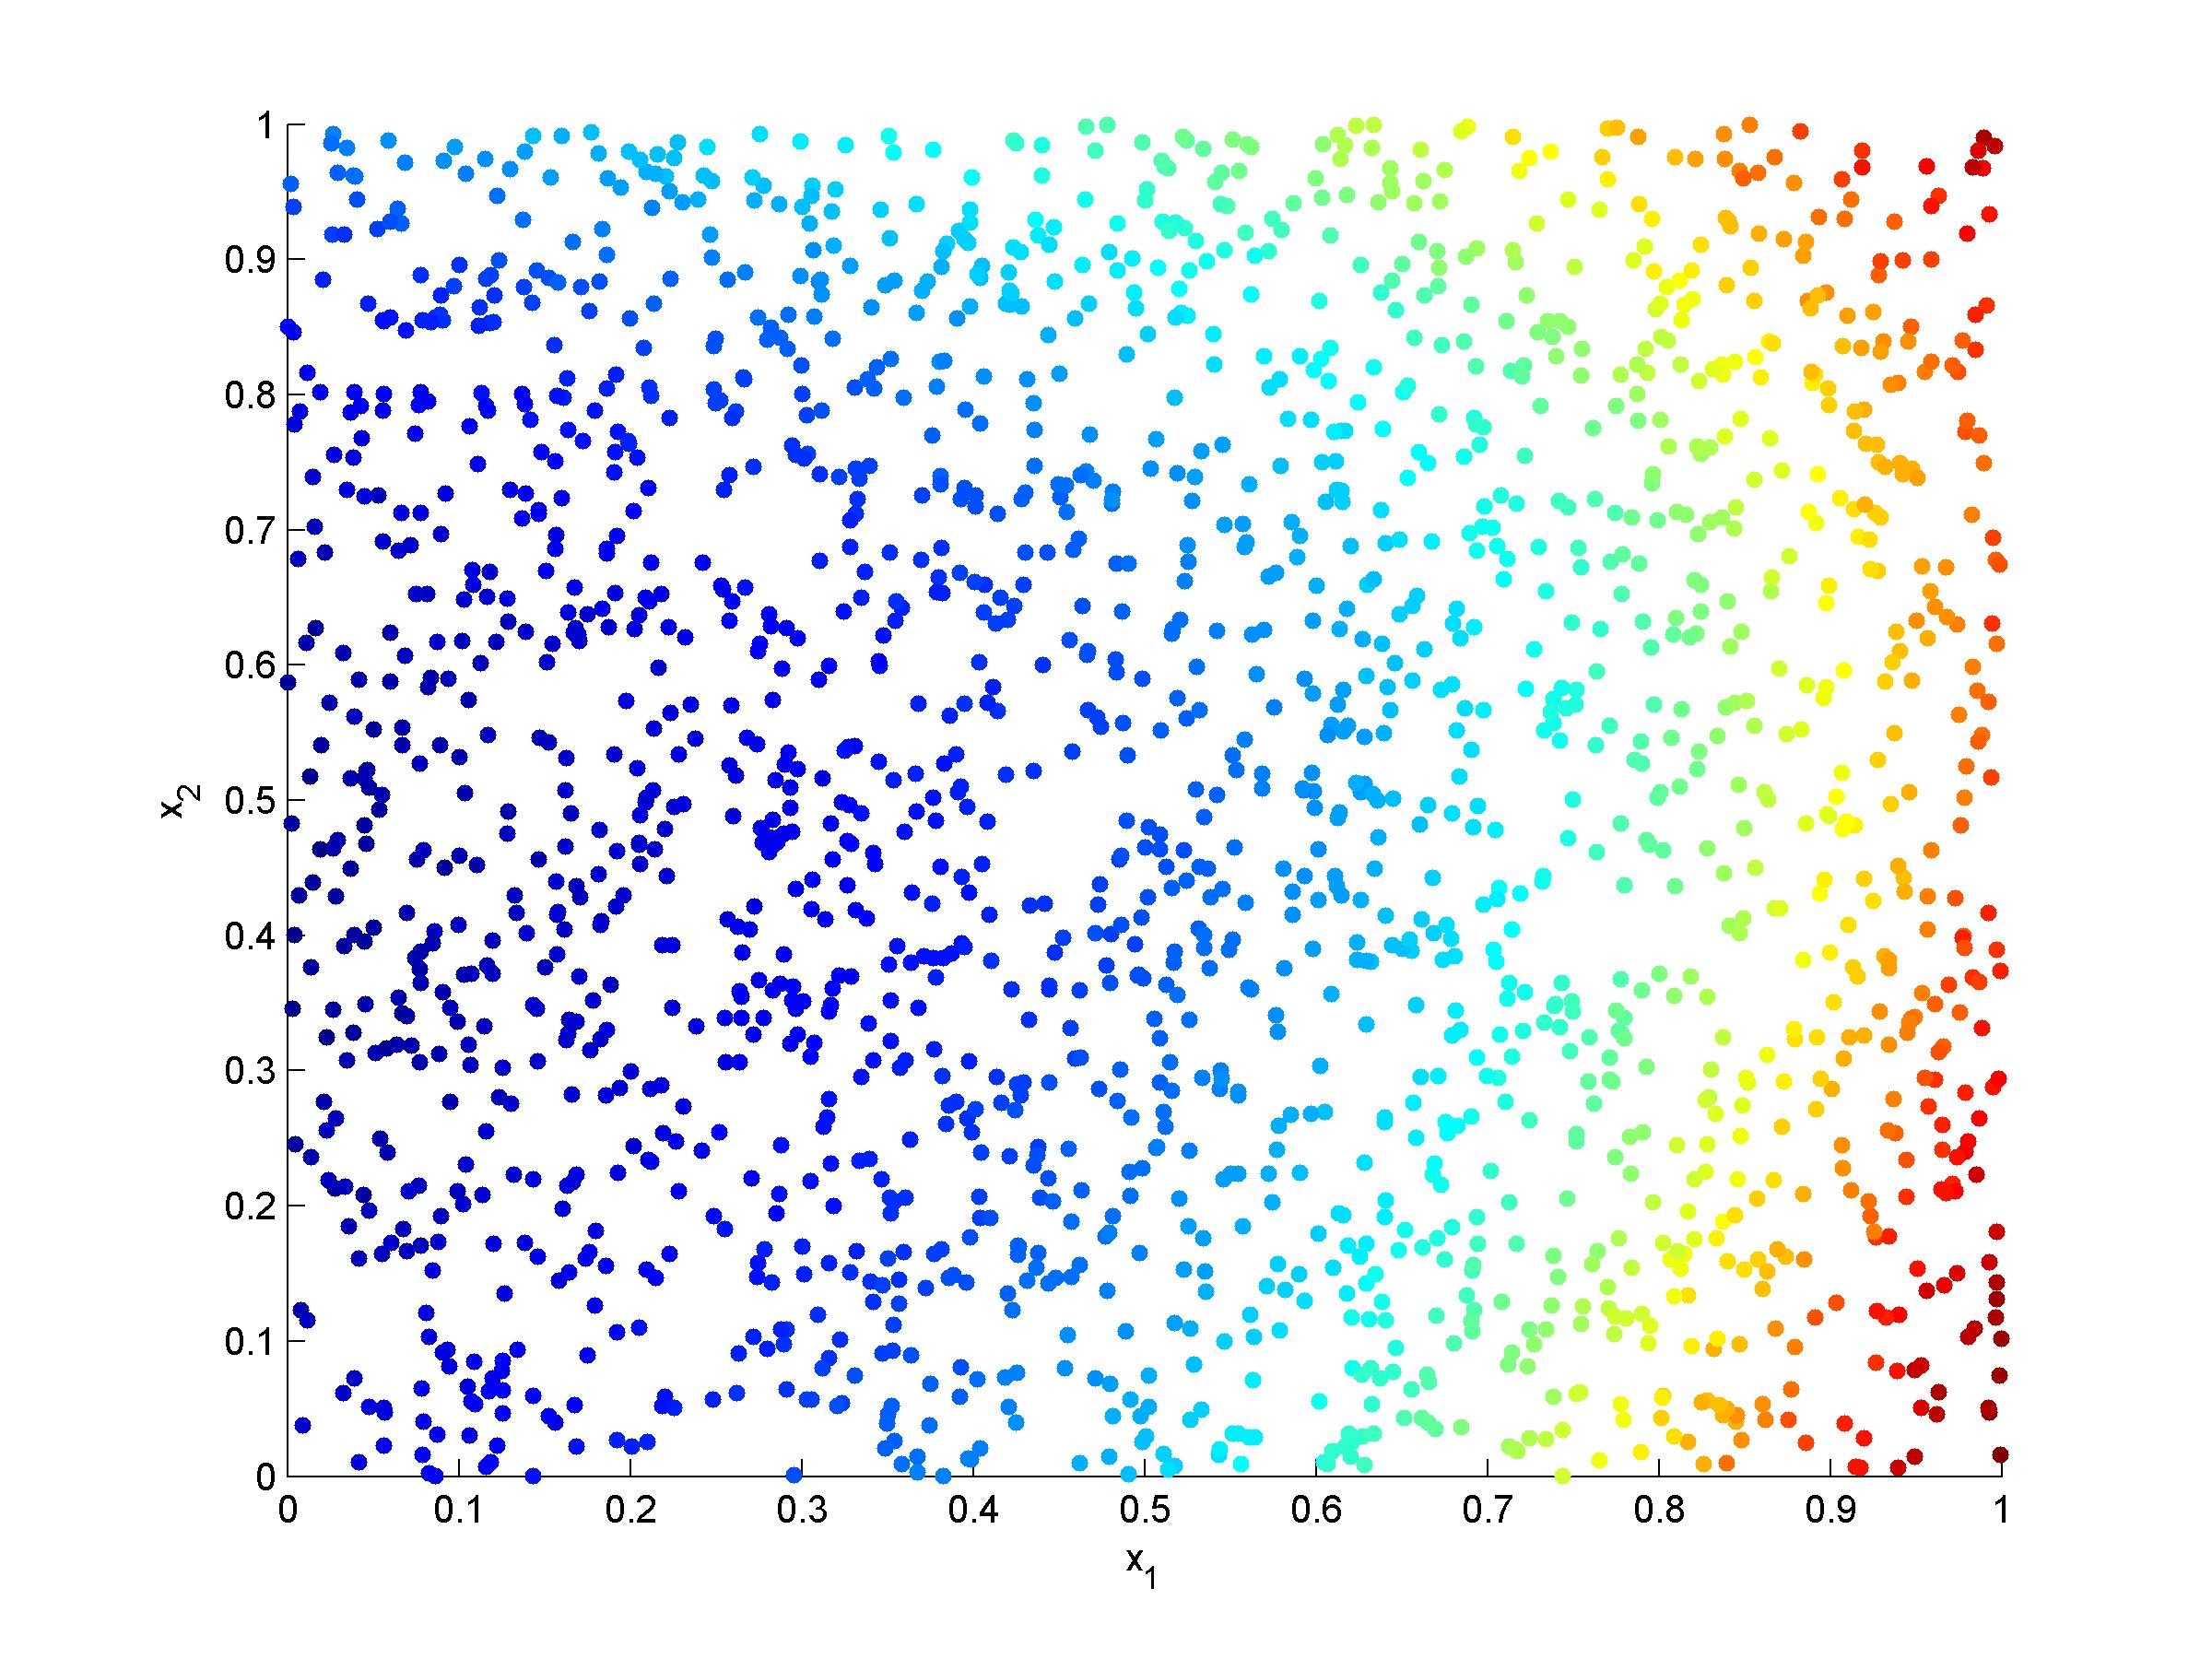
\includegraphics[width=0.5\textwidth]{xdata_noise2_colored_NIV2}
\caption{Data in ``true'' space ($x_1, x_2$), colored by the first (left) and second (right) nontrivial NIV. The NIV embedding is computed from the data in the ambient space with added noise ($z_1, z_2$, with $\sigma = 100$). Note that the parameterizations we obtain are not the eigenfunctions that we expect for points sampled from the unit square, but are now similar to the parameterizations obtained from DMAPS shown in Figure \ref{fig:xdata_dmaps}.}
\label{fig:xdata_NIV_noise2}
\end{figure}

\end{document}